\batchmode
\documentclass[a4paper]{book}
\usepackage{makeidx}
\usepackage{graphicx}
\usepackage{multicol}
\usepackage{float}
\usepackage{listings}
\usepackage{color}
\usepackage{ifthen}
\usepackage[table]{xcolor}
\usepackage{textcomp}
\usepackage{alltt}
\usepackage[utf8]{inputenc}
\usepackage{mathptmx}
\usepackage[scaled=.90]{helvet}
\usepackage{courier}
\usepackage{doxygen}
\lstset{language=C++,inputencoding=utf8,basicstyle=\footnotesize,breaklines=true,breakatwhitespace=true,tabsize=8,numbers=left }
\makeindex
\setcounter{tocdepth}{3}
\renewcommand{\footrulewidth}{0.4pt}
\begin{document}
\begin{titlepage}
\vspace*{7cm}
\begin{center}
{\Large teleop\_\-framework }\\
\vspace*{1cm}
{\large Generated by Doxygen 1.7.3}\\
\vspace*{0.5cm}
{\small Sat Feb 25 2012 04:55:40}\\
\end{center}
\end{titlepage}
\clearemptydoublepage
\pagenumbering{roman}
\tableofcontents
\clearemptydoublepage
\pagenumbering{arabic}
\chapter{Main Page}
\label{index} 
\chapter{Namespace Index}
\section{Namespace List}
Here is a list of all namespaces with brief descriptions:\begin{DoxyCompactList}
\item\contentsline{section}{{\bf ros} }{\pageref{namespaceros}}{}
\item\contentsline{section}{{\bf ros::message\_\-operations} }{\pageref{namespaceros_1_1message__operations}}{}
\item\contentsline{section}{{\bf ros::message\_\-traits} }{\pageref{namespaceros_1_1message__traits}}{}
\item\contentsline{section}{{\bf ros::serialization} }{\pageref{namespaceros_1_1serialization}}{}
\item\contentsline{section}{{\bf teleop\_\-msgs} }{\pageref{namespaceteleop__msgs}}{}
\item\contentsline{section}{{\bf teleop\_\-msgs::msg} }{\pageref{namespaceteleop__msgs_1_1msg}}{}
\item\contentsline{section}{{\bf teleop\_\-msgs::msg::\_\-Axis} }{\pageref{namespaceteleop__msgs_1_1msg_1_1__Axis}}{}
\item\contentsline{section}{{\bf teleop\_\-msgs::msg::\_\-Button} }{\pageref{namespaceteleop__msgs_1_1msg_1_1__Button}}{}
\item\contentsline{section}{{\bf teleop\_\-msgs::msg::\_\-State} }{\pageref{namespaceteleop__msgs_1_1msg_1_1__State}}{}
\end{DoxyCompactList}

\chapter{Class Index}
\section{Class List}
Here are the classes, structs, unions and interfaces with brief descriptions:\begin{DoxyCompactList}
\item\contentsline{section}{{\bf teleop::TeleopSourceJoystick} }{\pageref{classteleop_1_1TeleopSourceJoystick}}{}
\end{DoxyCompactList}

\chapter{File Index}
\section{File List}
Here is a list of all files with brief descriptions:\begin{DoxyCompactList}
\item\contentsline{section}{/home/klc/Code/github.com/teleop/teleop\_\-msgs/msg\_\-gen/cpp/include/teleop\_\-msgs/{\bf Axis.h} }{\pageref{Axis_8h}}{}
\item\contentsline{section}{/home/klc/Code/github.com/teleop/teleop\_\-msgs/msg\_\-gen/cpp/include/teleop\_\-msgs/{\bf Button.h} }{\pageref{Button_8h}}{}
\item\contentsline{section}{/home/klc/Code/github.com/teleop/teleop\_\-msgs/msg\_\-gen/cpp/include/teleop\_\-msgs/{\bf State.h} }{\pageref{State_8h}}{}
\item\contentsline{section}{/home/klc/Code/github.com/teleop/teleop\_\-msgs/src/teleop\_\-msgs/{\bf \_\-\_\-init\_\-\_\-.py} }{\pageref{____init_____8py}}{}
\item\contentsline{section}{/home/klc/Code/github.com/teleop/teleop\_\-msgs/src/teleop\_\-msgs/msg/{\bf \_\-\_\-init\_\-\_\-.py} }{\pageref{msg_2____init_____8py}}{}
\item\contentsline{section}{/home/klc/Code/github.com/teleop/teleop\_\-msgs/src/teleop\_\-msgs/msg/{\bf \_\-Axis.py} }{\pageref{__Axis_8py}}{}
\item\contentsline{section}{/home/klc/Code/github.com/teleop/teleop\_\-msgs/src/teleop\_\-msgs/msg/{\bf \_\-Button.py} }{\pageref{__Button_8py}}{}
\item\contentsline{section}{/home/klc/Code/github.com/teleop/teleop\_\-msgs/src/teleop\_\-msgs/msg/{\bf \_\-State.py} }{\pageref{__State_8py}}{}
\end{DoxyCompactList}

\chapter{Namespace Documentation}
\section{teleop Namespace Reference}
\label{namespaceteleop}\index{teleop@{teleop}}
\subsection*{Classes}
\begin{DoxyCompactItemize}
\item 
class {\bf TeleopSourceJoystick}
\end{DoxyCompactItemize}

\chapter{Class Documentation}
\section{teleop::TeleopAxis Struct Reference}
\label{structteleop_1_1TeleopAxis}\index{teleop::TeleopAxis@{teleop::TeleopAxis}}


{\ttfamily \#include $<$teleop\_\-common.hpp$>$}

\subsection*{Public Attributes}
\begin{DoxyCompactItemize}
\item 
{\bf TeleopAxisType} {\bf type}
\item 
{\bf TeleopAxisValue} {\bf value}
\end{DoxyCompactItemize}


\subsection{Detailed Description}
Teleop device axis (value is in [TELEOP\_\-AXIS\_\-MIN, TELEOP\_\-AXIS\_\-MAX]) 

Definition at line 118 of file teleop\_\-common.hpp.



\subsection{Member Data Documentation}
\index{teleop::TeleopAxis@{teleop::TeleopAxis}!type@{type}}
\index{type@{type}!teleop::TeleopAxis@{teleop::TeleopAxis}}
\subsubsection[{type}]{\setlength{\rightskip}{0pt plus 5cm}{\bf TeleopAxisType} {\bf teleop::TeleopAxis::type}}\label{structteleop_1_1TeleopAxis_a58fbf33e3c6d2adad996c1241f501d62}


Definition at line 119 of file teleop\_\-common.hpp.

\index{teleop::TeleopAxis@{teleop::TeleopAxis}!value@{value}}
\index{value@{value}!teleop::TeleopAxis@{teleop::TeleopAxis}}
\subsubsection[{value}]{\setlength{\rightskip}{0pt plus 5cm}{\bf TeleopAxisValue} {\bf teleop::TeleopAxis::value}}\label{structteleop_1_1TeleopAxis_a91054bd85c1385032673ab0c235a4c59}


Definition at line 120 of file teleop\_\-common.hpp.



The documentation for this struct was generated from the following file:\begin{DoxyCompactItemize}
\item 
/home/klc/Code/github.com/teleop/teleop\_\-framework/include/{\bf teleop\_\-common.hpp}\end{DoxyCompactItemize}

\section{teleop::TeleopButton Struct Reference}
\label{structteleop_1_1TeleopButton}\index{teleop::TeleopButton@{teleop::TeleopButton}}


{\ttfamily \#include $<$teleop\_\-common.hpp$>$}

\subsection*{Public Attributes}
\begin{DoxyCompactItemize}
\item 
{\bf TeleopButtonType} {\bf type}
\item 
{\bf TeleopButtonValue} {\bf value}
\end{DoxyCompactItemize}


\subsection{Detailed Description}
Teleop device button (value of 0 means off) 

Definition at line 124 of file teleop\_\-common.hpp.



\subsection{Member Data Documentation}
\index{teleop::TeleopButton@{teleop::TeleopButton}!type@{type}}
\index{type@{type}!teleop::TeleopButton@{teleop::TeleopButton}}
\subsubsection[{type}]{\setlength{\rightskip}{0pt plus 5cm}{\bf TeleopButtonType} {\bf teleop::TeleopButton::type}}\label{structteleop_1_1TeleopButton_ade22e95f36234e9a9e417adef318f92d}


Definition at line 125 of file teleop\_\-common.hpp.

\index{teleop::TeleopButton@{teleop::TeleopButton}!value@{value}}
\index{value@{value}!teleop::TeleopButton@{teleop::TeleopButton}}
\subsubsection[{value}]{\setlength{\rightskip}{0pt plus 5cm}{\bf TeleopButtonValue} {\bf teleop::TeleopButton::value}}\label{structteleop_1_1TeleopButton_a945881d364a8344b61a6515d765e8531}


Definition at line 126 of file teleop\_\-common.hpp.



The documentation for this struct was generated from the following file:\begin{DoxyCompactItemize}
\item 
{\bf teleop\_\-common.hpp}\end{DoxyCompactItemize}

\section{teleop::TeleopSource Class Reference}
\label{classteleop_1_1TeleopSource}\index{teleop::TeleopSource@{teleop::TeleopSource}}


{\ttfamily \#include $<$teleop\_\-source.hpp$>$}

\subsection*{Public Member Functions}
\begin{DoxyCompactItemize}
\item 
virtual bool {\bf init} ()=0
\item 
virtual bool {\bf listen} (unsigned int listenTimeout, {\bf TeleopState} $\ast$const teleopState, bool $\ast$updated)=0
\item 
virtual bool {\bf shutdown} ()=0
\item 
virtual {\bf $\sim$TeleopSource} ()
\end{DoxyCompactItemize}


\subsection{Detailed Description}
This class defines a simple low-\/level interface to teleop sources.

The \doxyref{init()}{p.}{classteleop_1_1TeleopSource_a7dff7881d778c2c25c81a3cacd5d21b8} and \doxyref{shutdown()}{p.}{classteleop_1_1TeleopSource_ac614e5667e191a537bfd66dbf05dcee6} methods control the life cycle of the object. Note that \doxyref{shutdown()}{p.}{classteleop_1_1TeleopSource_ac614e5667e191a537bfd66dbf05dcee6} is always called on destruction.

The \doxyref{listen()}{p.}{classteleop_1_1TeleopSource_aa1592ea03919cfb3f1c0e79d9b664507} method listens for teleop source events and updates the provided teleop state accordingly. 

Definition at line 68 of file teleop\_\-source.hpp.



\subsection{Constructor \& Destructor Documentation}
\index{teleop::TeleopSource@{teleop::TeleopSource}!$\sim$TeleopSource@{$\sim$TeleopSource}}
\index{$\sim$TeleopSource@{$\sim$TeleopSource}!teleop::TeleopSource@{teleop::TeleopSource}}
\subsubsection[{$\sim$TeleopSource}]{\setlength{\rightskip}{0pt plus 5cm}virtual teleop::TeleopSource::$\sim$TeleopSource (
\begin{DoxyParamCaption}
{}
\end{DoxyParamCaption}
)\hspace{0.3cm}{\ttfamily  [inline, virtual]}}\label{classteleop_1_1TeleopSource_a3c6c6e57c41b49b0dcda414dd5359112}
Destructor. Virtual so destruction will invoke sub-\/class destructor. 

Definition at line 75 of file teleop\_\-source.hpp.



\subsection{Member Function Documentation}
\index{teleop::TeleopSource@{teleop::TeleopSource}!init@{init}}
\index{init@{init}!teleop::TeleopSource@{teleop::TeleopSource}}
\subsubsection[{init}]{\setlength{\rightskip}{0pt plus 5cm}virtual bool teleop::TeleopSource::init (
\begin{DoxyParamCaption}
{}
\end{DoxyParamCaption}
)\hspace{0.3cm}{\ttfamily  [pure virtual]}}\label{classteleop_1_1TeleopSource_a7dff7881d778c2c25c81a3cacd5d21b8}
Initialise object (open files, etc.). If object is already initialised it is shutdown and reinitialised.

\begin{DoxyReturn}{Returns}
true on success 
\end{DoxyReturn}
\index{teleop::TeleopSource@{teleop::TeleopSource}!listen@{listen}}
\index{listen@{listen}!teleop::TeleopSource@{teleop::TeleopSource}}
\subsubsection[{listen}]{\setlength{\rightskip}{0pt plus 5cm}virtual bool teleop::TeleopSource::listen (
\begin{DoxyParamCaption}
\item[{unsigned int}]{listenTimeout, }
\item[{{\bf TeleopState} $\ast$const}]{teleopState, }
\item[{bool $\ast$}]{updated}
\end{DoxyParamCaption}
)\hspace{0.3cm}{\ttfamily  [pure virtual]}}\label{classteleop_1_1TeleopSource_aa1592ea03919cfb3f1c0e79d9b664507}
Blocks until teleop source device events detected or the given timeout is reached. When events occur, updates the teleop state. Should only be called between \doxyref{init()}{p.}{classteleop_1_1TeleopSource_a7dff7881d778c2c25c81a3cacd5d21b8} and \doxyref{shutdown()}{p.}{classteleop_1_1TeleopSource_ac614e5667e191a537bfd66dbf05dcee6}.


\begin{DoxyParams}{Parameters}
{\em listenTimeout} & [in] -\/ timeout value in milliseconds \\
\hline
{\em teleopState} & [in/out] -\/ the current teleop state, to be updated \\
\hline
{\em updated} & [out] -\/ true if teleop state was updated\\
\hline
\end{DoxyParams}
\begin{DoxyReturn}{Returns}
true on success 
\end{DoxyReturn}
\index{teleop::TeleopSource@{teleop::TeleopSource}!shutdown@{shutdown}}
\index{shutdown@{shutdown}!teleop::TeleopSource@{teleop::TeleopSource}}
\subsubsection[{shutdown}]{\setlength{\rightskip}{0pt plus 5cm}virtual bool teleop::TeleopSource::shutdown (
\begin{DoxyParamCaption}
{}
\end{DoxyParamCaption}
)\hspace{0.3cm}{\ttfamily  [pure virtual]}}\label{classteleop_1_1TeleopSource_ac614e5667e191a537bfd66dbf05dcee6}
Shutdown object (close files, etc.). If object is already shutdown this has no effect. This method always cleans up as much as possible, even if there are errors. This method is always called on destruction.

\begin{DoxyReturn}{Returns}
true on success 
\end{DoxyReturn}


The documentation for this class was generated from the following file:\begin{DoxyCompactItemize}
\item 
/home/klc/Code/github.com/teleop/teleop\_\-framework/include/{\bf teleop\_\-source.hpp}\end{DoxyCompactItemize}

\section{teleop::TeleopSourceAdapter Class Reference}
\label{classteleop_1_1TeleopSourceAdapter}\index{teleop::TeleopSourceAdapter@{teleop::TeleopSourceAdapter}}


{\ttfamily \#include $<$teleop\_\-source\_\-adapter.hpp$>$}

\subsection*{Classes}
\begin{DoxyCompactItemize}
\item 
class {\bf TeleopSourceAdapterCallback}
\end{DoxyCompactItemize}
\subsection*{Public Member Functions}
\begin{DoxyCompactItemize}
\item 
{\bf TeleopAxisValue} {\bf getAxisDeadZone} ({\bf TeleopAxisType} axisType)
\item 
bool {\bf getAxisInverted} ({\bf TeleopAxisType} axisType)
\item 
unsigned int {\bf getListenTimeout} ()
\item 
bool {\bf init} ({\bf TeleopSource} $\ast$teleopSource, {\bf TeleopSourceAdapterCallback} $\ast$callback)
\item 
bool {\bf isInitialised} ()
\item 
bool {\bf isListeningThread} ()
\item 
bool {\bf isRunning} ()
\item 
bool {\bf setAxisDeadZone} ({\bf TeleopAxisValue} axisDeadZone, {\bf TeleopAxisType} axisType)
\item 
bool {\bf setAxisDeadZoneForAllAxes} ({\bf TeleopAxisValue} axisDeadZone)
\item 
bool {\bf setAxisInverted} (bool axisInverted, {\bf TeleopAxisType} axisType)
\item 
bool {\bf setAxisInvertedForAllAxes} (bool axisInverted)
\item 
bool {\bf setListenTimeout} (unsigned int listenTimeout)
\item 
bool {\bf shutdown} ()
\item 
bool {\bf start} (bool blocking)
\item 
bool {\bf stop} (bool blocking)
\item 
{\bf TeleopSourceAdapter} ()
\item 
bool {\bf waitForStopped} ()
\item 
{\bf $\sim$TeleopSourceAdapter} ()
\end{DoxyCompactItemize}
\subsection*{Static Public Attributes}
\begin{DoxyCompactItemize}
\item 
static const {\bf TeleopAxisValue} {\bf AXIS\_\-DEAD\_\-ZONE\_\-DEFAULT} = 0.05
\item 
static const {\bf TeleopAxisValue} {\bf AXIS\_\-DEAD\_\-ZONE\_\-MAX} = 0.99
\item 
static const {\bf TeleopAxisValue} {\bf AXIS\_\-DEAD\_\-ZONE\_\-MIN} = 0.01
\item 
static const unsigned int {\bf LISTEN\_\-TIMEOUT\_\-DEFAULT} = 200
\end{DoxyCompactItemize}
\subsection*{Private Member Functions}
\begin{DoxyCompactItemize}
\item 
void {\bf listeningThread} ()
\end{DoxyCompactItemize}
\subsection*{Private Attributes}
\begin{DoxyCompactItemize}
\item 
{\bf TeleopAxisValue} {\bf mAxisDeadZone} [{\bf TELEOP\_\-AXIS\_\-TYPE\_\-COUNT}]
\item 
boost::mutex {\bf mAxisDeadZoneMutex}
\item 
bool {\bf mAxisInverted} [{\bf TELEOP\_\-AXIS\_\-TYPE\_\-COUNT}]
\item 
boost::mutex {\bf mAxisInvertedMutex}
\item 
{\bf TeleopSourceAdapterCallback} $\ast$ {\bf mCallback}
\item 
bool {\bf mIsInitialised}
\item 
boost::recursive\_\-mutex {\bf mIsInitialisedMutex}
\item 
bool {\bf mIsRunning}
\item 
boost::mutex {\bf mIsRunningMutex}
\item 
boost::thread {\bf mListeningThread}
\item 
unsigned int {\bf mListenTimeout}
\item 
boost::mutex {\bf mListenTimeoutMutex}
\item 
{\bf TeleopSource} $\ast$ {\bf mTeleopSource}
\end{DoxyCompactItemize}


\subsection{Detailed Description}
This class defines an adapter object used to provide high-\/level thread-\/based control of a given teleop source object.

The \doxyref{init()}{p.}{classteleop_1_1TeleopSourceAdapter_a2015a77728ce26515a7bf37a234cdc3d} and \doxyref{shutdown()}{p.}{classteleop_1_1TeleopSourceAdapter_a76ebc9ecd211a9539780edfddaeffa3d} methods control the life cycle of the object. Note that \doxyref{shutdown()}{p.}{classteleop_1_1TeleopSourceAdapter_a76ebc9ecd211a9539780edfddaeffa3d} is always called on destruction.

The \doxyref{start()}{p.}{classteleop_1_1TeleopSourceAdapter_a98e341938478434c34f50e554e028607} and \doxyref{stop()}{p.}{classteleop_1_1TeleopSourceAdapter_ad531b50253e9c4e5468340a03c77f608} methods start and stop a listening thread which listens for teleop device events and reports them using the updated() callback. When the listening thread is about to stop, the stopping() callback is called. The listening thread may stop due to a call to \doxyref{stop()}{p.}{classteleop_1_1TeleopSourceAdapter_ad531b50253e9c4e5468340a03c77f608}, an error, or destruction of the adapter object.

To wait for the listening thread to stop, the \doxyref{waitForStopped()}{p.}{classteleop_1_1TeleopSourceAdapter_a624f8f41a9aff80853116f0a804d3cda} method can be called; alternatively, the \doxyref{start()}{p.}{classteleop_1_1TeleopSourceAdapter_a98e341938478434c34f50e554e028607} and \doxyref{stop()}{p.}{classteleop_1_1TeleopSourceAdapter_ad531b50253e9c4e5468340a03c77f608} methods can be called in blocking mode. The stopping() callback is called before any of the blocking methods return. The blocking methods may return in any order.

Both callbacks are called from the listening thread. As such, calls to \doxyref{init()}{p.}{classteleop_1_1TeleopSourceAdapter_a2015a77728ce26515a7bf37a234cdc3d}, \doxyref{start()}{p.}{classteleop_1_1TeleopSourceAdapter_a98e341938478434c34f50e554e028607}, \doxyref{stop()}{p.}{classteleop_1_1TeleopSourceAdapter_ad531b50253e9c4e5468340a03c77f608}, and \doxyref{waitForStopped()}{p.}{classteleop_1_1TeleopSourceAdapter_a624f8f41a9aff80853116f0a804d3cda} will always fail when called from either callback. Calls to \doxyref{shutdown()}{p.}{classteleop_1_1TeleopSourceAdapter_a76ebc9ecd211a9539780edfddaeffa3d} or destruction of the adapter object from either callback are not permitted, and will cause the program to be aborted (to avoid undefined behaviour). 

Definition at line 84 of file teleop\_\-source\_\-adapter.hpp.



\subsection{Constructor \& Destructor Documentation}
\index{teleop::TeleopSourceAdapter@{teleop::TeleopSourceAdapter}!TeleopSourceAdapter@{TeleopSourceAdapter}}
\index{TeleopSourceAdapter@{TeleopSourceAdapter}!teleop::TeleopSourceAdapter@{teleop::TeleopSourceAdapter}}
\subsubsection[{TeleopSourceAdapter}]{\setlength{\rightskip}{0pt plus 5cm}teleop::TeleopSourceAdapter::TeleopSourceAdapter (
\begin{DoxyParamCaption}
{}
\end{DoxyParamCaption}
)}\label{classteleop_1_1TeleopSourceAdapter_a4de895719bf230b00b363c3d04d8f825}
Constructor. 

Definition at line 68 of file teleop\_\-source\_\-adapter.cpp.

\index{teleop::TeleopSourceAdapter@{teleop::TeleopSourceAdapter}!$\sim$TeleopSourceAdapter@{$\sim$TeleopSourceAdapter}}
\index{$\sim$TeleopSourceAdapter@{$\sim$TeleopSourceAdapter}!teleop::TeleopSourceAdapter@{teleop::TeleopSourceAdapter}}
\subsubsection[{$\sim$TeleopSourceAdapter}]{\setlength{\rightskip}{0pt plus 5cm}teleop::TeleopSourceAdapter::$\sim$TeleopSourceAdapter (
\begin{DoxyParamCaption}
{}
\end{DoxyParamCaption}
)}\label{classteleop_1_1TeleopSourceAdapter_aed47bdc6b6af58f315b507889e78e0ed}
Destructor. 

Definition at line 81 of file teleop\_\-source\_\-adapter.cpp.



\subsection{Member Function Documentation}
\index{teleop::TeleopSourceAdapter@{teleop::TeleopSourceAdapter}!getAxisDeadZone@{getAxisDeadZone}}
\index{getAxisDeadZone@{getAxisDeadZone}!teleop::TeleopSourceAdapter@{teleop::TeleopSourceAdapter}}
\subsubsection[{getAxisDeadZone}]{\setlength{\rightskip}{0pt plus 5cm}{\bf TeleopAxisValue} teleop::TeleopSourceAdapter::getAxisDeadZone (
\begin{DoxyParamCaption}
\item[{{\bf TeleopAxisType}}]{axisType}
\end{DoxyParamCaption}
)}\label{classteleop_1_1TeleopSourceAdapter_a208c97709902da783d172d62d32a56a6}
Get axis dead zone for a given axis.


\begin{DoxyParams}{Parameters}
{\em axisType} & [in] -\/ axis type\\
\hline
\end{DoxyParams}
\begin{DoxyReturn}{Returns}
axis dead zone 
\end{DoxyReturn}


Definition at line 396 of file teleop\_\-source\_\-adapter.cpp.

\index{teleop::TeleopSourceAdapter@{teleop::TeleopSourceAdapter}!getAxisInverted@{getAxisInverted}}
\index{getAxisInverted@{getAxisInverted}!teleop::TeleopSourceAdapter@{teleop::TeleopSourceAdapter}}
\subsubsection[{getAxisInverted}]{\setlength{\rightskip}{0pt plus 5cm}bool teleop::TeleopSourceAdapter::getAxisInverted (
\begin{DoxyParamCaption}
\item[{{\bf TeleopAxisType}}]{axisType}
\end{DoxyParamCaption}
)}\label{classteleop_1_1TeleopSourceAdapter_a88a7c0271354d068e01136c38323f005}
Get axis inverted status for a given axis.


\begin{DoxyParams}{Parameters}
{\em axisType} & [in] -\/ axis type\\
\hline
\end{DoxyParams}
\begin{DoxyReturn}{Returns}
axis inverted 
\end{DoxyReturn}


Definition at line 418 of file teleop\_\-source\_\-adapter.cpp.

\index{teleop::TeleopSourceAdapter@{teleop::TeleopSourceAdapter}!getListenTimeout@{getListenTimeout}}
\index{getListenTimeout@{getListenTimeout}!teleop::TeleopSourceAdapter@{teleop::TeleopSourceAdapter}}
\subsubsection[{getListenTimeout}]{\setlength{\rightskip}{0pt plus 5cm}unsigned int teleop::TeleopSourceAdapter::getListenTimeout (
\begin{DoxyParamCaption}
{}
\end{DoxyParamCaption}
)}\label{classteleop_1_1TeleopSourceAdapter_a76b3b632449d22a90bc4caad9b61cad3}
Get listen timeout, which specifies how often to check for interruption.

\begin{DoxyReturn}{Returns}
listen timeout in milliseconds 
\end{DoxyReturn}


Definition at line 362 of file teleop\_\-source\_\-adapter.cpp.

\index{teleop::TeleopSourceAdapter@{teleop::TeleopSourceAdapter}!init@{init}}
\index{init@{init}!teleop::TeleopSourceAdapter@{teleop::TeleopSourceAdapter}}
\subsubsection[{init}]{\setlength{\rightskip}{0pt plus 5cm}bool teleop::TeleopSourceAdapter::init (
\begin{DoxyParamCaption}
\item[{{\bf TeleopSource} $\ast$}]{teleopSource, }
\item[{{\bf TeleopSourceAdapterCallback} $\ast$}]{callback}
\end{DoxyParamCaption}
)}\label{classteleop_1_1TeleopSourceAdapter_a2015a77728ce26515a7bf37a234cdc3d}
Initialise object. If object is already initialised it is shutdown and reinitialised. After a successful call to this method the teleop source and callback objects should not be destroyed or shutdown until the \doxyref{shutdown()}{p.}{classteleop_1_1TeleopSourceAdapter_a76ebc9ecd211a9539780edfddaeffa3d} method has been called.


\begin{DoxyParams}{Parameters}
{\em teleopSource} & -\/ teleop source object to use \\
\hline
{\em callback} & -\/ callback object to use\\
\hline
\end{DoxyParams}
\begin{DoxyReturn}{Returns}
true on success 
\end{DoxyReturn}


Definition at line 95 of file teleop\_\-source\_\-adapter.cpp.

\index{teleop::TeleopSourceAdapter@{teleop::TeleopSourceAdapter}!isInitialised@{isInitialised}}
\index{isInitialised@{isInitialised}!teleop::TeleopSourceAdapter@{teleop::TeleopSourceAdapter}}
\subsubsection[{isInitialised}]{\setlength{\rightskip}{0pt plus 5cm}bool teleop::TeleopSourceAdapter::isInitialised (
\begin{DoxyParamCaption}
{}
\end{DoxyParamCaption}
)}\label{classteleop_1_1TeleopSourceAdapter_a4af3415218324ddf1c949133207fa212}
Check if node is initialised.

\begin{DoxyReturn}{Returns}
true if initialised 
\end{DoxyReturn}


Definition at line 259 of file teleop\_\-source\_\-adapter.cpp.

\index{teleop::TeleopSourceAdapter@{teleop::TeleopSourceAdapter}!isListeningThread@{isListeningThread}}
\index{isListeningThread@{isListeningThread}!teleop::TeleopSourceAdapter@{teleop::TeleopSourceAdapter}}
\subsubsection[{isListeningThread}]{\setlength{\rightskip}{0pt plus 5cm}bool teleop::TeleopSourceAdapter::isListeningThread (
\begin{DoxyParamCaption}
{}
\end{DoxyParamCaption}
)}\label{classteleop_1_1TeleopSourceAdapter_a9a7906e6b9437956aefada3aa767cc84}
Check if current thread is the listening thread.

\begin{DoxyReturn}{Returns}
true if this is the listening thread 
\end{DoxyReturn}


Definition at line 269 of file teleop\_\-source\_\-adapter.cpp.

\index{teleop::TeleopSourceAdapter@{teleop::TeleopSourceAdapter}!isRunning@{isRunning}}
\index{isRunning@{isRunning}!teleop::TeleopSourceAdapter@{teleop::TeleopSourceAdapter}}
\subsubsection[{isRunning}]{\setlength{\rightskip}{0pt plus 5cm}bool teleop::TeleopSourceAdapter::isRunning (
\begin{DoxyParamCaption}
{}
\end{DoxyParamCaption}
)}\label{classteleop_1_1TeleopSourceAdapter_ac43dc68d400ed3a0fa475b775ff2c091}
Check if node is running.

\begin{DoxyReturn}{Returns}
true if running 
\end{DoxyReturn}


Definition at line 264 of file teleop\_\-source\_\-adapter.cpp.

\index{teleop::TeleopSourceAdapter@{teleop::TeleopSourceAdapter}!listeningThread@{listeningThread}}
\index{listeningThread@{listeningThread}!teleop::TeleopSourceAdapter@{teleop::TeleopSourceAdapter}}
\subsubsection[{listeningThread}]{\setlength{\rightskip}{0pt plus 5cm}void teleop::TeleopSourceAdapter::listeningThread (
\begin{DoxyParamCaption}
{}
\end{DoxyParamCaption}
)\hspace{0.3cm}{\ttfamily  [private]}}\label{classteleop_1_1TeleopSourceAdapter_a7d12b25ae28324708f6df5c3186eb793}
Executes main listen loop (run in listening thread). 

Definition at line 277 of file teleop\_\-source\_\-adapter.cpp.

\index{teleop::TeleopSourceAdapter@{teleop::TeleopSourceAdapter}!setAxisDeadZone@{setAxisDeadZone}}
\index{setAxisDeadZone@{setAxisDeadZone}!teleop::TeleopSourceAdapter@{teleop::TeleopSourceAdapter}}
\subsubsection[{setAxisDeadZone}]{\setlength{\rightskip}{0pt plus 5cm}bool teleop::TeleopSourceAdapter::setAxisDeadZone (
\begin{DoxyParamCaption}
\item[{{\bf TeleopAxisValue}}]{axisDeadZone, }
\item[{{\bf TeleopAxisType}}]{axisType}
\end{DoxyParamCaption}
)}\label{classteleop_1_1TeleopSourceAdapter_a439ef27cd7020428be8115e8f510e34a}
Set axis dead zone for a given axis.


\begin{DoxyParams}{Parameters}
{\em axisDeadZone} & [in] -\/ axis dead zone \\
\hline
{\em axisType} & [in] -\/ axis type\\
\hline
\end{DoxyParams}
\begin{DoxyReturn}{Returns}
true on success 
\end{DoxyReturn}


Definition at line 383 of file teleop\_\-source\_\-adapter.cpp.

\index{teleop::TeleopSourceAdapter@{teleop::TeleopSourceAdapter}!setAxisDeadZoneForAllAxes@{setAxisDeadZoneForAllAxes}}
\index{setAxisDeadZoneForAllAxes@{setAxisDeadZoneForAllAxes}!teleop::TeleopSourceAdapter@{teleop::TeleopSourceAdapter}}
\subsubsection[{setAxisDeadZoneForAllAxes}]{\setlength{\rightskip}{0pt plus 5cm}bool teleop::TeleopSourceAdapter::setAxisDeadZoneForAllAxes (
\begin{DoxyParamCaption}
\item[{{\bf TeleopAxisValue}}]{axisDeadZone}
\end{DoxyParamCaption}
)}\label{classteleop_1_1TeleopSourceAdapter_adee00e2a68d1b0b69526646b5a962112}
Set axis dead zone for all axes.


\begin{DoxyParams}{Parameters}
{\em deadZone} & [in] -\/ axis dead zone\\
\hline
\end{DoxyParams}
\begin{DoxyReturn}{Returns}
true on success 
\end{DoxyReturn}


Definition at line 368 of file teleop\_\-source\_\-adapter.cpp.

\index{teleop::TeleopSourceAdapter@{teleop::TeleopSourceAdapter}!setAxisInverted@{setAxisInverted}}
\index{setAxisInverted@{setAxisInverted}!teleop::TeleopSourceAdapter@{teleop::TeleopSourceAdapter}}
\subsubsection[{setAxisInverted}]{\setlength{\rightskip}{0pt plus 5cm}bool teleop::TeleopSourceAdapter::setAxisInverted (
\begin{DoxyParamCaption}
\item[{bool}]{axisInverted, }
\item[{{\bf TeleopAxisType}}]{axisType}
\end{DoxyParamCaption}
)}\label{classteleop_1_1TeleopSourceAdapter_accc3f630e85ca2668a80c1da4a730c66}
Set axis inverted status for a given axis.


\begin{DoxyParams}{Parameters}
{\em axisInverted} & [in] -\/ axis inverted status \\
\hline
{\em axisType} & [in] -\/ axis type\\
\hline
\end{DoxyParams}
\begin{DoxyReturn}{Returns}
true on success 
\end{DoxyReturn}


Definition at line 411 of file teleop\_\-source\_\-adapter.cpp.

\index{teleop::TeleopSourceAdapter@{teleop::TeleopSourceAdapter}!setAxisInvertedForAllAxes@{setAxisInvertedForAllAxes}}
\index{setAxisInvertedForAllAxes@{setAxisInvertedForAllAxes}!teleop::TeleopSourceAdapter@{teleop::TeleopSourceAdapter}}
\subsubsection[{setAxisInvertedForAllAxes}]{\setlength{\rightskip}{0pt plus 5cm}bool teleop::TeleopSourceAdapter::setAxisInvertedForAllAxes (
\begin{DoxyParamCaption}
\item[{bool}]{axisInverted}
\end{DoxyParamCaption}
)}\label{classteleop_1_1TeleopSourceAdapter_a8253d2657dd53c24384396a3e1be9a6a}
Set axis inverted status for all axes.


\begin{DoxyParams}{Parameters}
{\em axisInverted} & [in] -\/ axis inverted status\\
\hline
\end{DoxyParams}
\begin{DoxyReturn}{Returns}
true on success 
\end{DoxyReturn}


Definition at line 402 of file teleop\_\-source\_\-adapter.cpp.

\index{teleop::TeleopSourceAdapter@{teleop::TeleopSourceAdapter}!setListenTimeout@{setListenTimeout}}
\index{setListenTimeout@{setListenTimeout}!teleop::TeleopSourceAdapter@{teleop::TeleopSourceAdapter}}
\subsubsection[{setListenTimeout}]{\setlength{\rightskip}{0pt plus 5cm}bool teleop::TeleopSourceAdapter::setListenTimeout (
\begin{DoxyParamCaption}
\item[{unsigned int}]{listenTimeout}
\end{DoxyParamCaption}
)}\label{classteleop_1_1TeleopSourceAdapter_ac7acc3e5e3f2edf4a0c0d496bd5bdf23}
Set listen timeout, which specifies how often to check for interruption.


\begin{DoxyParams}{Parameters}
{\em listenTimeout} & [in] -\/ listen timeout in milliseconds\\
\hline
\end{DoxyParams}
\begin{DoxyReturn}{Returns}
true on success 
\end{DoxyReturn}


Definition at line 355 of file teleop\_\-source\_\-adapter.cpp.

\index{teleop::TeleopSourceAdapter@{teleop::TeleopSourceAdapter}!shutdown@{shutdown}}
\index{shutdown@{shutdown}!teleop::TeleopSourceAdapter@{teleop::TeleopSourceAdapter}}
\subsubsection[{shutdown}]{\setlength{\rightskip}{0pt plus 5cm}bool teleop::TeleopSourceAdapter::shutdown (
\begin{DoxyParamCaption}
{}
\end{DoxyParamCaption}
)}\label{classteleop_1_1TeleopSourceAdapter_a76ebc9ecd211a9539780edfddaeffa3d}
Shutdown object. If object is already shutdown this has no effect. This method always cleans up as much as possible, even if there are errors. This method is always called on destruction.

\begin{DoxyReturn}{Returns}
true on success 
\end{DoxyReturn}


Definition at line 128 of file teleop\_\-source\_\-adapter.cpp.

\index{teleop::TeleopSourceAdapter@{teleop::TeleopSourceAdapter}!start@{start}}
\index{start@{start}!teleop::TeleopSourceAdapter@{teleop::TeleopSourceAdapter}}
\subsubsection[{start}]{\setlength{\rightskip}{0pt plus 5cm}bool teleop::TeleopSourceAdapter::start (
\begin{DoxyParamCaption}
\item[{bool}]{blocking}
\end{DoxyParamCaption}
)}\label{classteleop_1_1TeleopSourceAdapter_a98e341938478434c34f50e554e028607}
Start listening thread. If listening thread is already running this has no effect, although it will block if the blocking flag is set. Should only be called between \doxyref{init()}{p.}{classteleop_1_1TeleopSourceAdapter_a2015a77728ce26515a7bf37a234cdc3d} and \doxyref{shutdown()}{p.}{classteleop_1_1TeleopSourceAdapter_a76ebc9ecd211a9539780edfddaeffa3d}.


\begin{DoxyParams}{Parameters}
{\em blocking} & -\/ if true block until stopped\\
\hline
\end{DoxyParams}
\begin{DoxyReturn}{Returns}
true on success (or already running) 
\end{DoxyReturn}


Definition at line 158 of file teleop\_\-source\_\-adapter.cpp.

\index{teleop::TeleopSourceAdapter@{teleop::TeleopSourceAdapter}!stop@{stop}}
\index{stop@{stop}!teleop::TeleopSourceAdapter@{teleop::TeleopSourceAdapter}}
\subsubsection[{stop}]{\setlength{\rightskip}{0pt plus 5cm}bool teleop::TeleopSourceAdapter::stop (
\begin{DoxyParamCaption}
\item[{bool}]{blocking}
\end{DoxyParamCaption}
)}\label{classteleop_1_1TeleopSourceAdapter_ad531b50253e9c4e5468340a03c77f608}
Request that the listening thread be stopped. If the listening thread is not running this has no effect. Should only be called between \doxyref{init()}{p.}{classteleop_1_1TeleopSourceAdapter_a2015a77728ce26515a7bf37a234cdc3d} and \doxyref{shutdown()}{p.}{classteleop_1_1TeleopSourceAdapter_a76ebc9ecd211a9539780edfddaeffa3d}.


\begin{DoxyParams}{Parameters}
{\em blocking} & -\/ if true block until stopped\\
\hline
\end{DoxyParams}
\begin{DoxyReturn}{Returns}
true on success (or already stopped) 
\end{DoxyReturn}


Definition at line 200 of file teleop\_\-source\_\-adapter.cpp.

\index{teleop::TeleopSourceAdapter@{teleop::TeleopSourceAdapter}!waitForStopped@{waitForStopped}}
\index{waitForStopped@{waitForStopped}!teleop::TeleopSourceAdapter@{teleop::TeleopSourceAdapter}}
\subsubsection[{waitForStopped}]{\setlength{\rightskip}{0pt plus 5cm}bool teleop::TeleopSourceAdapter::waitForStopped (
\begin{DoxyParamCaption}
{}
\end{DoxyParamCaption}
)}\label{classteleop_1_1TeleopSourceAdapter_a624f8f41a9aff80853116f0a804d3cda}
Block until teleop source is stopped. Should only be called between \doxyref{init()}{p.}{classteleop_1_1TeleopSourceAdapter_a2015a77728ce26515a7bf37a234cdc3d} and \doxyref{shutdown()}{p.}{classteleop_1_1TeleopSourceAdapter_a76ebc9ecd211a9539780edfddaeffa3d}.

\begin{DoxyReturn}{Returns}
true on success 
\end{DoxyReturn}


Definition at line 236 of file teleop\_\-source\_\-adapter.cpp.



\subsection{Member Data Documentation}
\index{teleop::TeleopSourceAdapter@{teleop::TeleopSourceAdapter}!AXIS\_\-DEAD\_\-ZONE\_\-DEFAULT@{AXIS\_\-DEAD\_\-ZONE\_\-DEFAULT}}
\index{AXIS\_\-DEAD\_\-ZONE\_\-DEFAULT@{AXIS\_\-DEAD\_\-ZONE\_\-DEFAULT}!teleop::TeleopSourceAdapter@{teleop::TeleopSourceAdapter}}
\subsubsection[{AXIS\_\-DEAD\_\-ZONE\_\-DEFAULT}]{\setlength{\rightskip}{0pt plus 5cm}const {\bf TeleopAxisValue} {\bf teleop::TeleopSourceAdapter::AXIS\_\-DEAD\_\-ZONE\_\-DEFAULT} = 0.05\hspace{0.3cm}{\ttfamily  [static]}}\label{classteleop_1_1TeleopSourceAdapter_afd4444eebb19bb0363d3da7dcd559bc1}
Axis dead zone default -\/ values smaller than dead zone are set to 0.0 

Definition at line 129 of file teleop\_\-source\_\-adapter.hpp.

\index{teleop::TeleopSourceAdapter@{teleop::TeleopSourceAdapter}!AXIS\_\-DEAD\_\-ZONE\_\-MAX@{AXIS\_\-DEAD\_\-ZONE\_\-MAX}}
\index{AXIS\_\-DEAD\_\-ZONE\_\-MAX@{AXIS\_\-DEAD\_\-ZONE\_\-MAX}!teleop::TeleopSourceAdapter@{teleop::TeleopSourceAdapter}}
\subsubsection[{AXIS\_\-DEAD\_\-ZONE\_\-MAX}]{\setlength{\rightskip}{0pt plus 5cm}const {\bf TeleopAxisValue} {\bf teleop::TeleopSourceAdapter::AXIS\_\-DEAD\_\-ZONE\_\-MAX} = 0.99\hspace{0.3cm}{\ttfamily  [static]}}\label{classteleop_1_1TeleopSourceAdapter_a609150532eb1309842ac7c9713e6c74e}
Axis dead zone max 

Definition at line 133 of file teleop\_\-source\_\-adapter.hpp.

\index{teleop::TeleopSourceAdapter@{teleop::TeleopSourceAdapter}!AXIS\_\-DEAD\_\-ZONE\_\-MIN@{AXIS\_\-DEAD\_\-ZONE\_\-MIN}}
\index{AXIS\_\-DEAD\_\-ZONE\_\-MIN@{AXIS\_\-DEAD\_\-ZONE\_\-MIN}!teleop::TeleopSourceAdapter@{teleop::TeleopSourceAdapter}}
\subsubsection[{AXIS\_\-DEAD\_\-ZONE\_\-MIN}]{\setlength{\rightskip}{0pt plus 5cm}const {\bf TeleopAxisValue} {\bf teleop::TeleopSourceAdapter::AXIS\_\-DEAD\_\-ZONE\_\-MIN} = 0.01\hspace{0.3cm}{\ttfamily  [static]}}\label{classteleop_1_1TeleopSourceAdapter_afb159eb407a444dd0b81a2cdf71b245c}
Axis dead zone min 

Definition at line 131 of file teleop\_\-source\_\-adapter.hpp.

\index{teleop::TeleopSourceAdapter@{teleop::TeleopSourceAdapter}!LISTEN\_\-TIMEOUT\_\-DEFAULT@{LISTEN\_\-TIMEOUT\_\-DEFAULT}}
\index{LISTEN\_\-TIMEOUT\_\-DEFAULT@{LISTEN\_\-TIMEOUT\_\-DEFAULT}!teleop::TeleopSourceAdapter@{teleop::TeleopSourceAdapter}}
\subsubsection[{LISTEN\_\-TIMEOUT\_\-DEFAULT}]{\setlength{\rightskip}{0pt plus 5cm}const unsigned int {\bf teleop::TeleopSourceAdapter::LISTEN\_\-TIMEOUT\_\-DEFAULT} = 200\hspace{0.3cm}{\ttfamily  [static]}}\label{classteleop_1_1TeleopSourceAdapter_a842873978d9af74b61eaea2bf5e1680d}
Listen timeout in milliseconds -\/ check for interruption this often 

Definition at line 126 of file teleop\_\-source\_\-adapter.hpp.

\index{teleop::TeleopSourceAdapter@{teleop::TeleopSourceAdapter}!mAxisDeadZone@{mAxisDeadZone}}
\index{mAxisDeadZone@{mAxisDeadZone}!teleop::TeleopSourceAdapter@{teleop::TeleopSourceAdapter}}
\subsubsection[{mAxisDeadZone}]{\setlength{\rightskip}{0pt plus 5cm}{\bf TeleopAxisValue} {\bf teleop::TeleopSourceAdapter::mAxisDeadZone}[{\bf TELEOP\_\-AXIS\_\-TYPE\_\-COUNT}]\hspace{0.3cm}{\ttfamily  [private]}}\label{classteleop_1_1TeleopSourceAdapter_a365542d3d5298c46845f925fcb69dc98}
Axis dead zones -\/ values smaller than this are set to 0.0 

Definition at line 308 of file teleop\_\-source\_\-adapter.hpp.

\index{teleop::TeleopSourceAdapter@{teleop::TeleopSourceAdapter}!mAxisDeadZoneMutex@{mAxisDeadZoneMutex}}
\index{mAxisDeadZoneMutex@{mAxisDeadZoneMutex}!teleop::TeleopSourceAdapter@{teleop::TeleopSourceAdapter}}
\subsubsection[{mAxisDeadZoneMutex}]{\setlength{\rightskip}{0pt plus 5cm}boost::mutex {\bf teleop::TeleopSourceAdapter::mAxisDeadZoneMutex}\hspace{0.3cm}{\ttfamily  [private]}}\label{classteleop_1_1TeleopSourceAdapter_ab8953dbd119c9ad306b062beea3bec9f}
Mutex to protect axis dead zone 

Definition at line 326 of file teleop\_\-source\_\-adapter.hpp.

\index{teleop::TeleopSourceAdapter@{teleop::TeleopSourceAdapter}!mAxisInverted@{mAxisInverted}}
\index{mAxisInverted@{mAxisInverted}!teleop::TeleopSourceAdapter@{teleop::TeleopSourceAdapter}}
\subsubsection[{mAxisInverted}]{\setlength{\rightskip}{0pt plus 5cm}bool {\bf teleop::TeleopSourceAdapter::mAxisInverted}[{\bf TELEOP\_\-AXIS\_\-TYPE\_\-COUNT}]\hspace{0.3cm}{\ttfamily  [private]}}\label{classteleop_1_1TeleopSourceAdapter_ade8213d8ff962028cb93a3688b063a21}
Axis inverted statuses -\/ true means axis values should be inverted 

Definition at line 311 of file teleop\_\-source\_\-adapter.hpp.

\index{teleop::TeleopSourceAdapter@{teleop::TeleopSourceAdapter}!mAxisInvertedMutex@{mAxisInvertedMutex}}
\index{mAxisInvertedMutex@{mAxisInvertedMutex}!teleop::TeleopSourceAdapter@{teleop::TeleopSourceAdapter}}
\subsubsection[{mAxisInvertedMutex}]{\setlength{\rightskip}{0pt plus 5cm}boost::mutex {\bf teleop::TeleopSourceAdapter::mAxisInvertedMutex}\hspace{0.3cm}{\ttfamily  [private]}}\label{classteleop_1_1TeleopSourceAdapter_adb3bba897cf3a7525282e39fdd088a7f}
Mutex to protect axis inverted 

Definition at line 329 of file teleop\_\-source\_\-adapter.hpp.

\index{teleop::TeleopSourceAdapter@{teleop::TeleopSourceAdapter}!mCallback@{mCallback}}
\index{mCallback@{mCallback}!teleop::TeleopSourceAdapter@{teleop::TeleopSourceAdapter}}
\subsubsection[{mCallback}]{\setlength{\rightskip}{0pt plus 5cm}{\bf TeleopSourceAdapterCallback}$\ast$ {\bf teleop::TeleopSourceAdapter::mCallback}\hspace{0.3cm}{\ttfamily  [private]}}\label{classteleop_1_1TeleopSourceAdapter_a3089c2691157e6873227a0b6e12dbaad}
Callback 

Definition at line 296 of file teleop\_\-source\_\-adapter.hpp.

\index{teleop::TeleopSourceAdapter@{teleop::TeleopSourceAdapter}!mIsInitialised@{mIsInitialised}}
\index{mIsInitialised@{mIsInitialised}!teleop::TeleopSourceAdapter@{teleop::TeleopSourceAdapter}}
\subsubsection[{mIsInitialised}]{\setlength{\rightskip}{0pt plus 5cm}bool {\bf teleop::TeleopSourceAdapter::mIsInitialised}\hspace{0.3cm}{\ttfamily  [private]}}\label{classteleop_1_1TeleopSourceAdapter_af6337632f751a88f2072f96c7b0ad495}
Init done flag 

Definition at line 299 of file teleop\_\-source\_\-adapter.hpp.

\index{teleop::TeleopSourceAdapter@{teleop::TeleopSourceAdapter}!mIsInitialisedMutex@{mIsInitialisedMutex}}
\index{mIsInitialisedMutex@{mIsInitialisedMutex}!teleop::TeleopSourceAdapter@{teleop::TeleopSourceAdapter}}
\subsubsection[{mIsInitialisedMutex}]{\setlength{\rightskip}{0pt plus 5cm}boost::recursive\_\-mutex {\bf teleop::TeleopSourceAdapter::mIsInitialisedMutex}\hspace{0.3cm}{\ttfamily  [private]}}\label{classteleop_1_1TeleopSourceAdapter_a7daa9ee08218d22655654bb1bc55bd0d}
Mutex to protect is initialised flag 

Definition at line 317 of file teleop\_\-source\_\-adapter.hpp.

\index{teleop::TeleopSourceAdapter@{teleop::TeleopSourceAdapter}!mIsRunning@{mIsRunning}}
\index{mIsRunning@{mIsRunning}!teleop::TeleopSourceAdapter@{teleop::TeleopSourceAdapter}}
\subsubsection[{mIsRunning}]{\setlength{\rightskip}{0pt plus 5cm}bool {\bf teleop::TeleopSourceAdapter::mIsRunning}\hspace{0.3cm}{\ttfamily  [private]}}\label{classteleop_1_1TeleopSourceAdapter_aca413c4675a7a9cc05ffc57caf671e25}
Is running flag 

Definition at line 302 of file teleop\_\-source\_\-adapter.hpp.

\index{teleop::TeleopSourceAdapter@{teleop::TeleopSourceAdapter}!mIsRunningMutex@{mIsRunningMutex}}
\index{mIsRunningMutex@{mIsRunningMutex}!teleop::TeleopSourceAdapter@{teleop::TeleopSourceAdapter}}
\subsubsection[{mIsRunningMutex}]{\setlength{\rightskip}{0pt plus 5cm}boost::mutex {\bf teleop::TeleopSourceAdapter::mIsRunningMutex}\hspace{0.3cm}{\ttfamily  [private]}}\label{classteleop_1_1TeleopSourceAdapter_a562f1e92a5e1058397274ad07d573ff4}
Mutex to protect is running flag 

Definition at line 320 of file teleop\_\-source\_\-adapter.hpp.

\index{teleop::TeleopSourceAdapter@{teleop::TeleopSourceAdapter}!mListeningThread@{mListeningThread}}
\index{mListeningThread@{mListeningThread}!teleop::TeleopSourceAdapter@{teleop::TeleopSourceAdapter}}
\subsubsection[{mListeningThread}]{\setlength{\rightskip}{0pt plus 5cm}boost::thread {\bf teleop::TeleopSourceAdapter::mListeningThread}\hspace{0.3cm}{\ttfamily  [private]}}\label{classteleop_1_1TeleopSourceAdapter_af3c4ab5d57d14f9499deec23333b9966}
Listening thread 

Definition at line 314 of file teleop\_\-source\_\-adapter.hpp.

\index{teleop::TeleopSourceAdapter@{teleop::TeleopSourceAdapter}!mListenTimeout@{mListenTimeout}}
\index{mListenTimeout@{mListenTimeout}!teleop::TeleopSourceAdapter@{teleop::TeleopSourceAdapter}}
\subsubsection[{mListenTimeout}]{\setlength{\rightskip}{0pt plus 5cm}unsigned int {\bf teleop::TeleopSourceAdapter::mListenTimeout}\hspace{0.3cm}{\ttfamily  [private]}}\label{classteleop_1_1TeleopSourceAdapter_a3408bb87e319a79523c19aa53afbf79f}
Listen timeout in milliseconds -\/ check for interruption this often 

Definition at line 305 of file teleop\_\-source\_\-adapter.hpp.

\index{teleop::TeleopSourceAdapter@{teleop::TeleopSourceAdapter}!mListenTimeoutMutex@{mListenTimeoutMutex}}
\index{mListenTimeoutMutex@{mListenTimeoutMutex}!teleop::TeleopSourceAdapter@{teleop::TeleopSourceAdapter}}
\subsubsection[{mListenTimeoutMutex}]{\setlength{\rightskip}{0pt plus 5cm}boost::mutex {\bf teleop::TeleopSourceAdapter::mListenTimeoutMutex}\hspace{0.3cm}{\ttfamily  [private]}}\label{classteleop_1_1TeleopSourceAdapter_a10f5c85088a089cf5d091bb5cc7eabe8}
Mutex to protect listen timeout 

Definition at line 323 of file teleop\_\-source\_\-adapter.hpp.

\index{teleop::TeleopSourceAdapter@{teleop::TeleopSourceAdapter}!mTeleopSource@{mTeleopSource}}
\index{mTeleopSource@{mTeleopSource}!teleop::TeleopSourceAdapter@{teleop::TeleopSourceAdapter}}
\subsubsection[{mTeleopSource}]{\setlength{\rightskip}{0pt plus 5cm}{\bf TeleopSource}$\ast$ {\bf teleop::TeleopSourceAdapter::mTeleopSource}\hspace{0.3cm}{\ttfamily  [private]}}\label{classteleop_1_1TeleopSourceAdapter_a27724752a0d3da16521a24e309f6ad02}
Teleop source 

Definition at line 293 of file teleop\_\-source\_\-adapter.hpp.



The documentation for this class was generated from the following files:\begin{DoxyCompactItemize}
\item 
/home/klc/Code/github.com/teleop/teleop\_\-framework/include/{\bf teleop\_\-source\_\-adapter.hpp}\item 
/home/klc/Code/github.com/teleop/teleop\_\-framework/src/{\bf teleop\_\-source\_\-adapter.cpp}\end{DoxyCompactItemize}

\section{teleop::TeleopSourceAdapter::TeleopSourceAdapterCallback Class Reference}
\label{classteleop_1_1TeleopSourceAdapter_1_1TeleopSourceAdapterCallback}\index{teleop::TeleopSourceAdapter::TeleopSourceAdapterCallback@{teleop::TeleopSourceAdapter::TeleopSourceAdapterCallback}}


{\ttfamily \#include $<$teleop\_\-source\_\-adapter.hpp$>$}

\subsection*{Public Member Functions}
\begin{DoxyCompactItemize}
\item 
virtual void {\bf stopping} (bool error)=0
\item 
virtual void {\bf updated} (const {\bf TeleopState} $\ast$const teleopState, bool stopping, bool error)=0
\item 
virtual {\bf $\sim$TeleopSourceAdapterCallback} ()
\end{DoxyCompactItemize}


\subsection{Detailed Description}
Callback class which reports teleop state updates and listening thread termination. Users should sub-\/class this to handle events. 

Definition at line 92 of file teleop\_\-source\_\-adapter.hpp.



\subsection{Constructor \& Destructor Documentation}
\index{teleop::TeleopSourceAdapter::TeleopSourceAdapterCallback@{teleop::TeleopSourceAdapter::TeleopSourceAdapterCallback}!$\sim$TeleopSourceAdapterCallback@{$\sim$TeleopSourceAdapterCallback}}
\index{$\sim$TeleopSourceAdapterCallback@{$\sim$TeleopSourceAdapterCallback}!teleop::TeleopSourceAdapter::TeleopSourceAdapterCallback@{teleop::TeleopSourceAdapter::TeleopSourceAdapterCallback}}
\subsubsection[{$\sim$TeleopSourceAdapterCallback}]{\setlength{\rightskip}{0pt plus 5cm}virtual teleop::TeleopSourceAdapter::TeleopSourceAdapterCallback::$\sim$TeleopSourceAdapterCallback (
\begin{DoxyParamCaption}
{}
\end{DoxyParamCaption}
)\hspace{0.3cm}{\ttfamily  [inline, virtual]}}\label{classteleop_1_1TeleopSourceAdapter_1_1TeleopSourceAdapterCallback_a1f93f61980400d325379c88d7626064f}
Destructor. Virtual so destruction will invoke sub-\/class destructor. 

Definition at line 99 of file teleop\_\-source\_\-adapter.hpp.



\subsection{Member Function Documentation}
\index{teleop::TeleopSourceAdapter::TeleopSourceAdapterCallback@{teleop::TeleopSourceAdapter::TeleopSourceAdapterCallback}!stopping@{stopping}}
\index{stopping@{stopping}!teleop::TeleopSourceAdapter::TeleopSourceAdapterCallback@{teleop::TeleopSourceAdapter::TeleopSourceAdapterCallback}}
\subsubsection[{stopping}]{\setlength{\rightskip}{0pt plus 5cm}virtual void teleop::TeleopSourceAdapter::TeleopSourceAdapterCallback::stopping (
\begin{DoxyParamCaption}
\item[{bool}]{error}
\end{DoxyParamCaption}
)\hspace{0.3cm}{\ttfamily  [pure virtual]}}\label{classteleop_1_1TeleopSourceAdapter_1_1TeleopSourceAdapterCallback_a2f4680bfd6d0df62b8edcfef09d0220b}
Callback used to report that the listening thread is stopping. This is called from the listening thread. The listening thread may be stopping due to a call to \doxyref{stop()}{p.}{classteleop_1_1TeleopSourceAdapter_ad531b50253e9c4e5468340a03c77f608}, an error, or destruction of the adapter object.


\begin{DoxyParams}{Parameters}
{\em error} & [in] -\/ true if stopping due to an error \\
\hline
\end{DoxyParams}
\index{teleop::TeleopSourceAdapter::TeleopSourceAdapterCallback@{teleop::TeleopSourceAdapter::TeleopSourceAdapterCallback}!updated@{updated}}
\index{updated@{updated}!teleop::TeleopSourceAdapter::TeleopSourceAdapterCallback@{teleop::TeleopSourceAdapter::TeleopSourceAdapterCallback}}
\subsubsection[{updated}]{\setlength{\rightskip}{0pt plus 5cm}virtual void teleop::TeleopSourceAdapter::TeleopSourceAdapterCallback::updated (
\begin{DoxyParamCaption}
\item[{const {\bf TeleopState} $\ast$const}]{teleopState, }
\item[{bool}]{stopping, }
\item[{bool}]{error}
\end{DoxyParamCaption}
)\hspace{0.3cm}{\ttfamily  [pure virtual]}}\label{classteleop_1_1TeleopSourceAdapter_1_1TeleopSourceAdapterCallback_a3d117cc350755bf68cba4f1ca1f4c7fa}
Callback used to report an updated teleop state. This is called from the listening thread. As such, this method should return quickly, to avoid delaying or even losing teleop events. An alternative could be to create a new thread for each call, but this could cause performance, buffering and synchronisation problems.


\begin{DoxyParams}{Parameters}
{\em teleopState} & [in] -\/ the latest teleop state \\
\hline
{\em stopping} & [in] -\/ true if listening thread is stopping \\
\hline
{\em error} & [in] -\/ true if there were errors while listening \\
\hline
\end{DoxyParams}


The documentation for this class was generated from the following file:\begin{DoxyCompactItemize}
\item 
/home/klc/Code/github.com/teleop/teleop\_\-framework/include/{\bf teleop\_\-source\_\-adapter.hpp}\end{DoxyCompactItemize}

\section{teleop::TeleopState Struct Reference}
\label{structteleop_1_1TeleopState}\index{teleop::TeleopState@{teleop::TeleopState}}


{\ttfamily \#include $<$teleop\_\-common.hpp$>$}

\subsection*{Public Attributes}
\begin{DoxyCompactItemize}
\item 
std::vector$<$ {\bf TeleopAxis} $>$ {\bf axes}
\item 
std::vector$<$ {\bf TeleopButton} $>$ {\bf buttons}
\end{DoxyCompactItemize}


\subsection{Detailed Description}
Teleop device state 

Definition at line 130 of file teleop\_\-common.hpp.



\subsection{Member Data Documentation}
\index{teleop::TeleopState@{teleop::TeleopState}!axes@{axes}}
\index{axes@{axes}!teleop::TeleopState@{teleop::TeleopState}}
\subsubsection[{axes}]{\setlength{\rightskip}{0pt plus 5cm}std::vector$<${\bf TeleopAxis}$>$ {\bf teleop::TeleopState::axes}}\label{structteleop_1_1TeleopState_a0d5d8ad57cb592bb92087febfbe56c3f}


Definition at line 131 of file teleop\_\-common.hpp.

\index{teleop::TeleopState@{teleop::TeleopState}!buttons@{buttons}}
\index{buttons@{buttons}!teleop::TeleopState@{teleop::TeleopState}}
\subsubsection[{buttons}]{\setlength{\rightskip}{0pt plus 5cm}std::vector$<${\bf TeleopButton}$>$ {\bf teleop::TeleopState::buttons}}\label{structteleop_1_1TeleopState_a547375b52aee503d2d22d9013d3952e6}


Definition at line 132 of file teleop\_\-common.hpp.



The documentation for this struct was generated from the following file:\begin{DoxyCompactItemize}
\item 
{\bf teleop\_\-common.hpp}\end{DoxyCompactItemize}

\chapter{File Documentation}
\section{/home/klc/Code/github.com/teleop/teleop\_\-framework/include/teleop\_\-common.hpp File Reference}
\label{teleop__common_8hpp}\index{/home/klc/Code/github.com/teleop/teleop\_\-framework/include/teleop\_\-common.hpp@{/home/klc/Code/github.com/teleop/teleop\_\-framework/include/teleop\_\-common.hpp}}
{\ttfamily \#include $<$vector$>$}\par
{\ttfamily \#include $<$string$>$}\par
Include dependency graph for teleop\_\-common.hpp:
\nopagebreak
\begin{figure}[H]
\begin{center}
\leavevmode
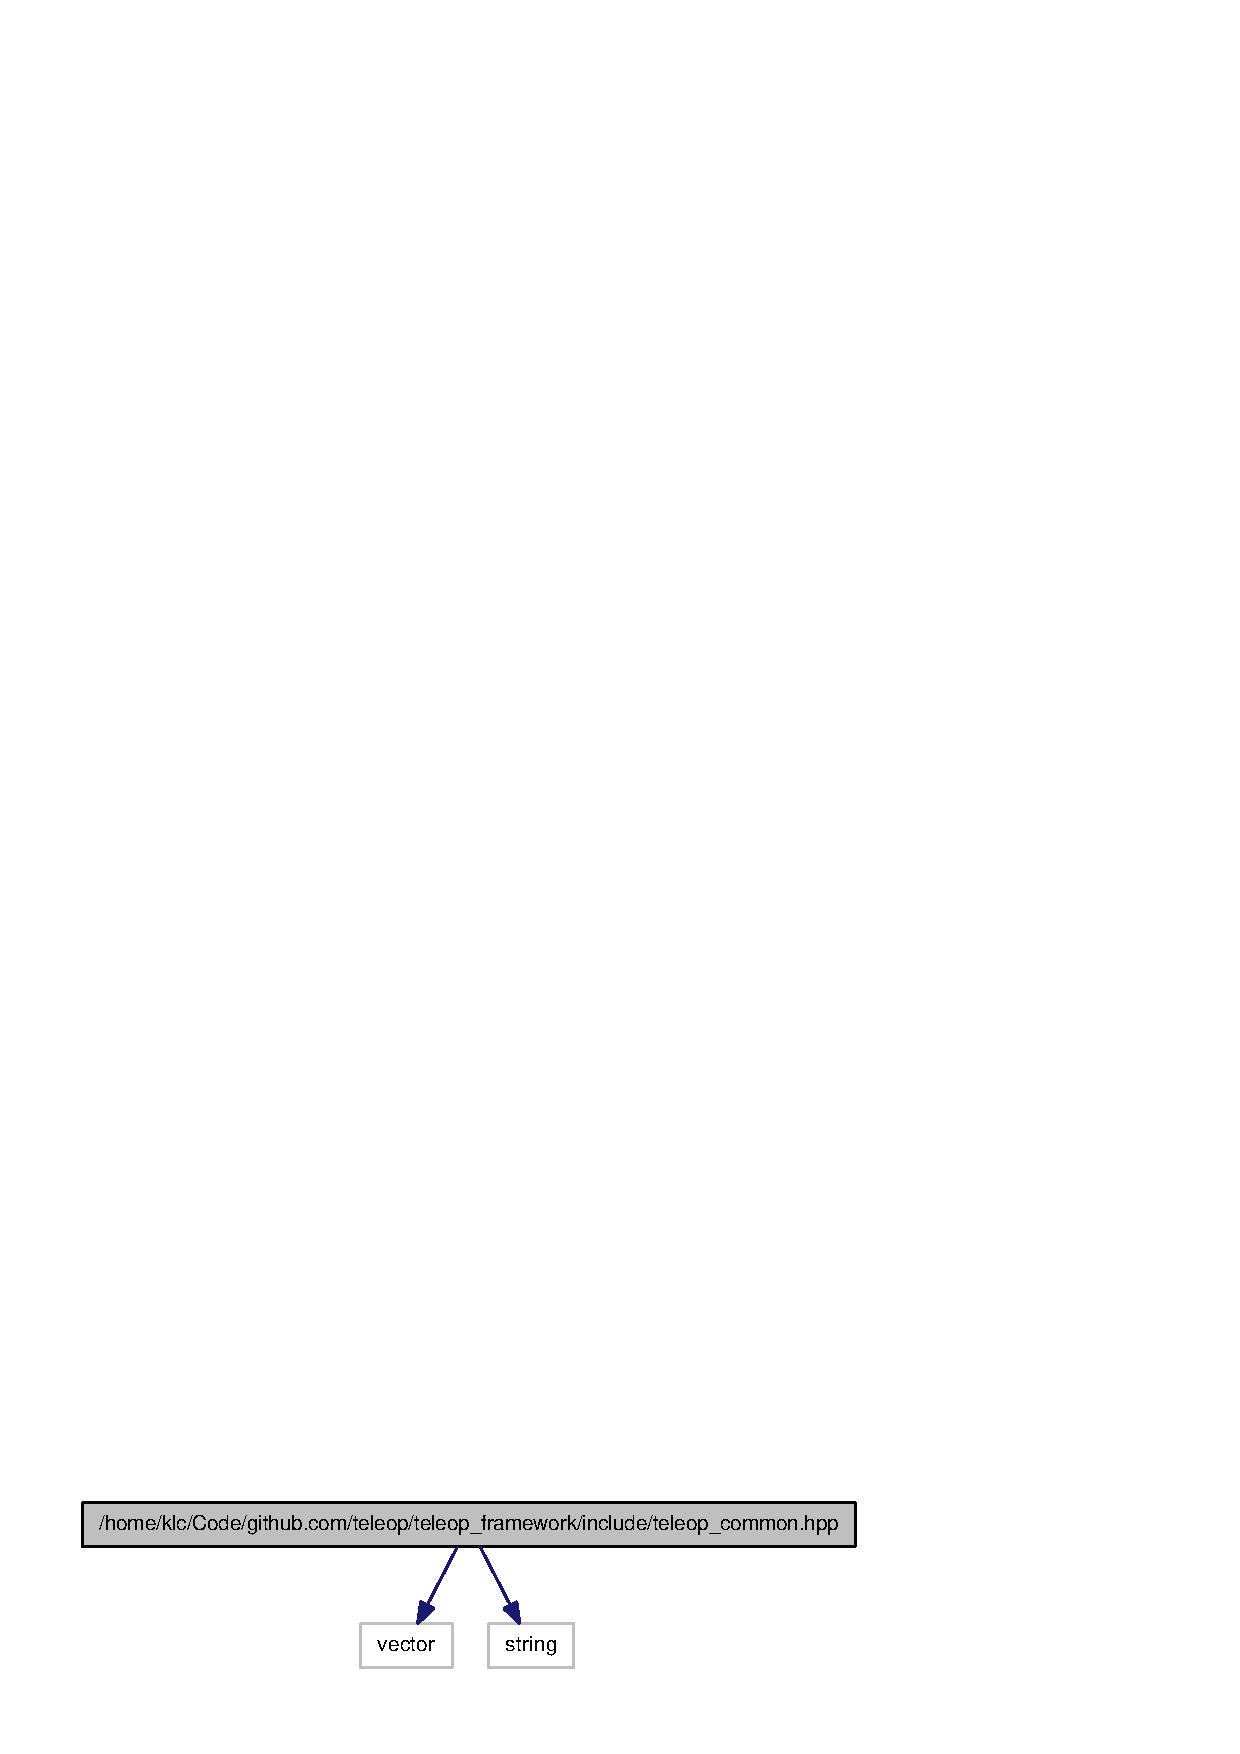
\includegraphics[width=400pt]{teleop__common_8hpp__incl}
\end{center}
\end{figure}
This graph shows which files directly or indirectly include this file:
\nopagebreak
\begin{figure}[H]
\begin{center}
\leavevmode
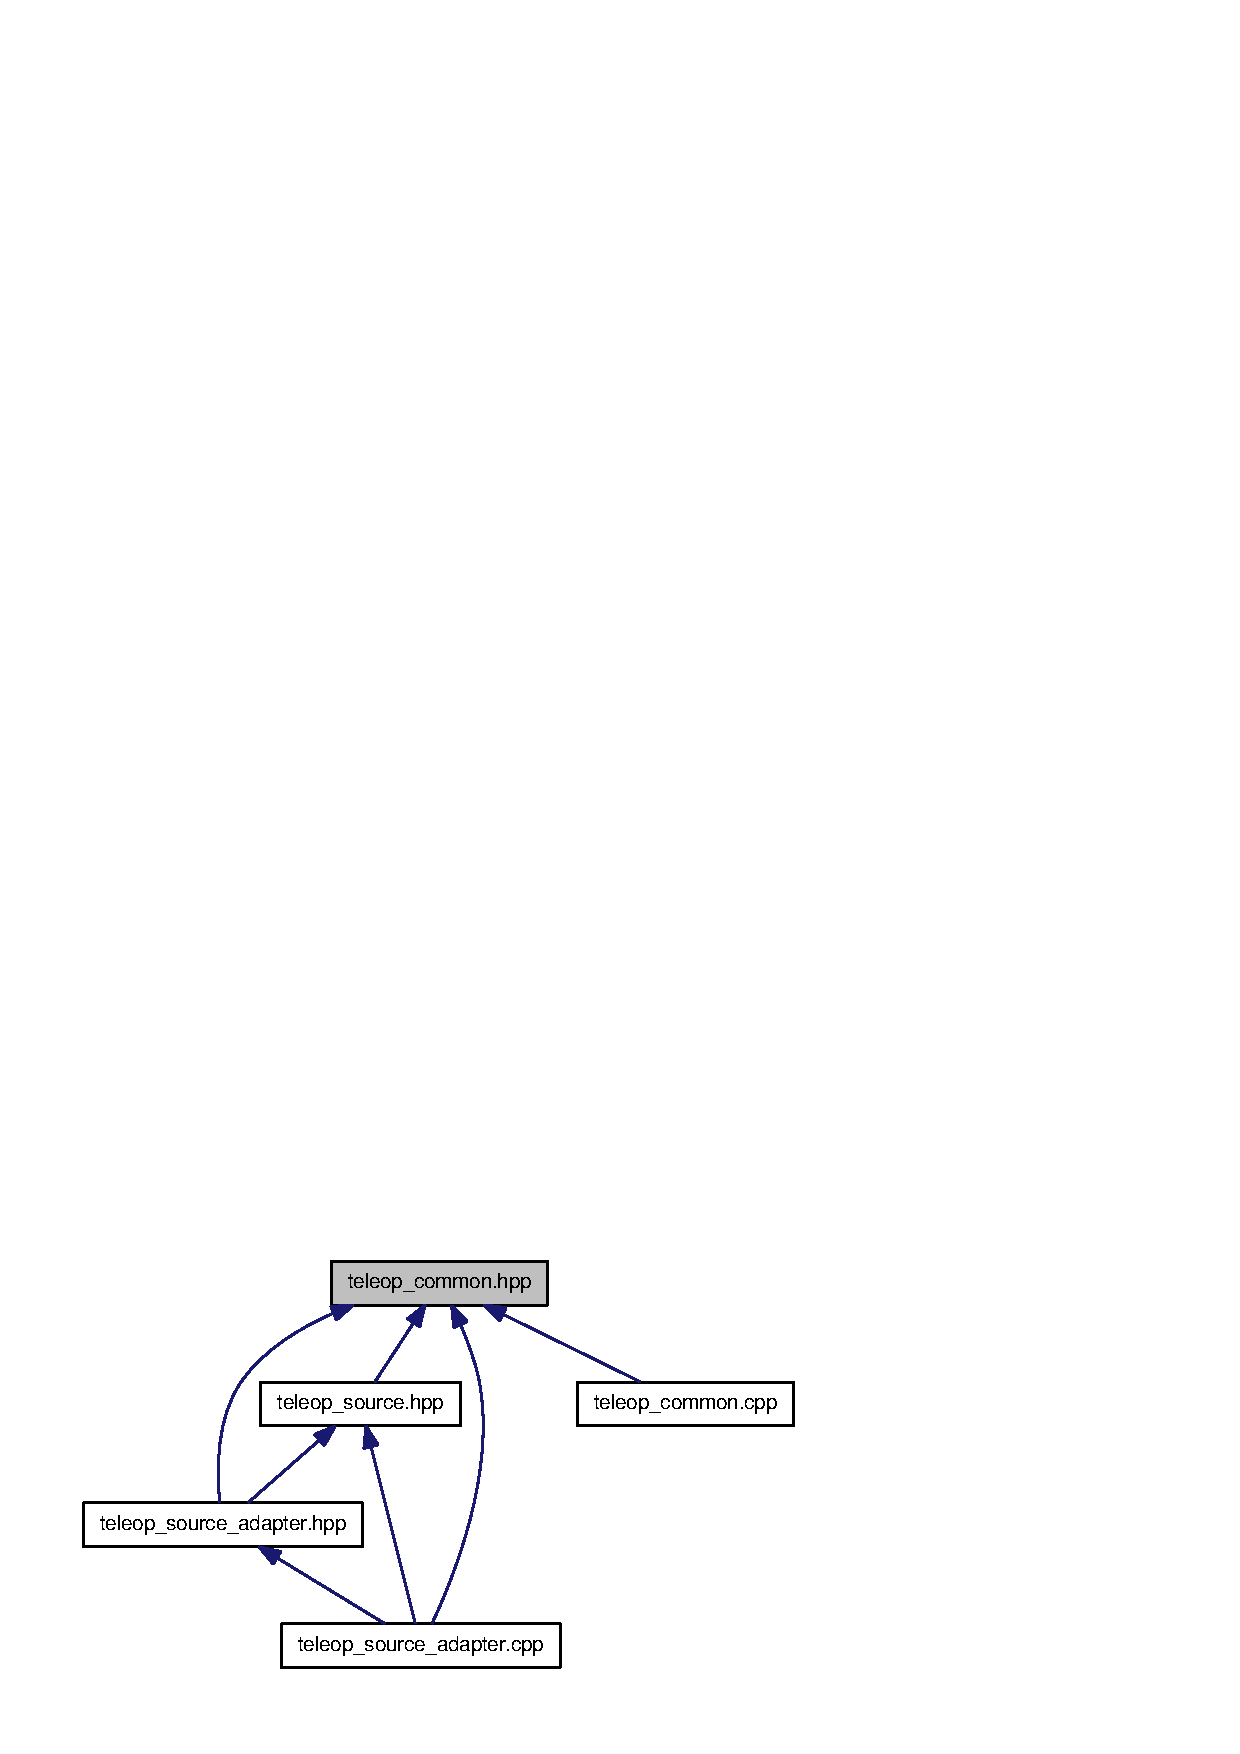
\includegraphics[width=400pt]{teleop__common_8hpp__dep__incl}
\end{center}
\end{figure}
\subsection*{Classes}
\begin{DoxyCompactItemize}
\item 
struct {\bf teleop::TeleopAxis}
\item 
struct {\bf teleop::TeleopButton}
\item 
struct {\bf teleop::TeleopState}
\end{DoxyCompactItemize}
\subsection*{Namespaces}
\begin{DoxyCompactItemize}
\item 
namespace {\bf teleop}
\end{DoxyCompactItemize}
\subsection*{Typedefs}
\begin{DoxyCompactItemize}
\item 
typedef double {\bf teleop::TeleopAxisValue}
\item 
typedef int {\bf teleop::TeleopButtonValue}
\end{DoxyCompactItemize}
\subsection*{Enumerations}
\begin{DoxyCompactItemize}
\item 
enum {\bf teleop::TeleopAxisType} \{ \par
{\bf teleop::TELEOP\_\-AXIS\_\-TYPE\_\-FIRST} =  0, 
{\bf teleop::TELEOP\_\-AXIS\_\-TYPE\_\-LIN\_\-X} =  TELEOP\_\-AXIS\_\-TYPE\_\-FIRST, 
{\bf teleop::TELEOP\_\-AXIS\_\-TYPE\_\-LIN\_\-Y}, 
{\bf teleop::TELEOP\_\-AXIS\_\-TYPE\_\-LIN\_\-Z}, 
\par
{\bf teleop::TELEOP\_\-AXIS\_\-TYPE\_\-ROT\_\-X}, 
{\bf teleop::TELEOP\_\-AXIS\_\-TYPE\_\-ROT\_\-Y}, 
{\bf teleop::TELEOP\_\-AXIS\_\-TYPE\_\-ROT\_\-Z}, 
{\bf teleop::TELEOP\_\-AXIS\_\-TYPE\_\-HAT0\_\-X}, 
\par
{\bf teleop::TELEOP\_\-AXIS\_\-TYPE\_\-HAT0\_\-Y}, 
{\bf teleop::TELEOP\_\-AXIS\_\-TYPE\_\-HAT1\_\-X}, 
{\bf teleop::TELEOP\_\-AXIS\_\-TYPE\_\-HAT1\_\-Y}, 
{\bf teleop::TELEOP\_\-AXIS\_\-TYPE\_\-HAT2\_\-X}, 
\par
{\bf teleop::TELEOP\_\-AXIS\_\-TYPE\_\-HAT2\_\-Y}, 
{\bf teleop::TELEOP\_\-AXIS\_\-TYPE\_\-HAT3\_\-X}, 
{\bf teleop::TELEOP\_\-AXIS\_\-TYPE\_\-HAT3\_\-Y}, 
{\bf teleop::TELEOP\_\-AXIS\_\-TYPE\_\-THROTTLE}, 
\par
{\bf teleop::TELEOP\_\-AXIS\_\-TYPE\_\-UNKNOWN}, 
{\bf teleop::TELEOP\_\-AXIS\_\-TYPE\_\-LAST} =  TELEOP\_\-AXIS\_\-TYPE\_\-UNKNOWN
 \}
\item 
enum {\bf teleop::TeleopButtonType} \{ \par
{\bf teleop::TELEOP\_\-BUTTON\_\-TYPE\_\-FIRST} =  0, 
{\bf teleop::TELEOP\_\-BUTTON\_\-TYPE\_\-0} =  TELEOP\_\-BUTTON\_\-TYPE\_\-FIRST, 
{\bf teleop::TELEOP\_\-BUTTON\_\-TYPE\_\-1}, 
{\bf teleop::TELEOP\_\-BUTTON\_\-TYPE\_\-2}, 
\par
{\bf teleop::TELEOP\_\-BUTTON\_\-TYPE\_\-3}, 
{\bf teleop::TELEOP\_\-BUTTON\_\-TYPE\_\-4}, 
{\bf teleop::TELEOP\_\-BUTTON\_\-TYPE\_\-5}, 
{\bf teleop::TELEOP\_\-BUTTON\_\-TYPE\_\-6}, 
\par
{\bf teleop::TELEOP\_\-BUTTON\_\-TYPE\_\-7}, 
{\bf teleop::TELEOP\_\-BUTTON\_\-TYPE\_\-8}, 
{\bf teleop::TELEOP\_\-BUTTON\_\-TYPE\_\-9}, 
{\bf teleop::TELEOP\_\-BUTTON\_\-TYPE\_\-A}, 
\par
{\bf teleop::TELEOP\_\-BUTTON\_\-TYPE\_\-B}, 
{\bf teleop::TELEOP\_\-BUTTON\_\-TYPE\_\-C}, 
{\bf teleop::TELEOP\_\-BUTTON\_\-TYPE\_\-X}, 
{\bf teleop::TELEOP\_\-BUTTON\_\-TYPE\_\-Y}, 
\par
{\bf teleop::TELEOP\_\-BUTTON\_\-TYPE\_\-Z}, 
{\bf teleop::TELEOP\_\-BUTTON\_\-TYPE\_\-RIGHT}, 
{\bf teleop::TELEOP\_\-BUTTON\_\-TYPE\_\-LEFT}, 
{\bf teleop::TELEOP\_\-BUTTON\_\-TYPE\_\-SELECT}, 
\par
{\bf teleop::TELEOP\_\-BUTTON\_\-TYPE\_\-START}, 
{\bf teleop::TELEOP\_\-BUTTON\_\-TYPE\_\-STOP}, 
{\bf teleop::TELEOP\_\-BUTTON\_\-TYPE\_\-TRIGGER}, 
{\bf teleop::TELEOP\_\-BUTTON\_\-TYPE\_\-UNKNOWN}, 
\par
{\bf teleop::TELEOP\_\-BUTTON\_\-TYPE\_\-LAST} =  TELEOP\_\-BUTTON\_\-TYPE\_\-UNKNOWN
 \}
\end{DoxyCompactItemize}
\subsection*{Functions}
\begin{DoxyCompactItemize}
\item 
std::string {\bf teleop::teleopAxisName} (TeleopAxisType axisType)
\item 
std::string {\bf teleop::teleopButtonName} (TeleopButtonType buttonType)
\end{DoxyCompactItemize}
\subsection*{Variables}
\begin{DoxyCompactItemize}
\item 
static const TeleopAxisValue {\bf teleop::TELEOP\_\-AXIS\_\-MAX} = 1.0
\item 
static const TeleopAxisValue {\bf teleop::TELEOP\_\-AXIS\_\-MIN} = -\/1.0
\item 
static const int {\bf teleop::TELEOP\_\-AXIS\_\-TYPE\_\-COUNT} = (TELEOP\_\-AXIS\_\-TYPE\_\-LAST -\/ TELEOP\_\-AXIS\_\-TYPE\_\-FIRST + 1)
\item 
static const int {\bf teleop::TELEOP\_\-BUTTON\_\-TYPE\_\-COUNT} = (TELEOP\_\-BUTTON\_\-TYPE\_\-LAST -\/ TELEOP\_\-BUTTON\_\-TYPE\_\-FIRST + 1)
\end{DoxyCompactItemize}

\section{teleop\_\-source.hpp File Reference}
\label{teleop__source_8hpp}\index{teleop\_\-source.hpp@{teleop\_\-source.hpp}}
{\ttfamily \#include $<$teleop\_\-common.hpp$>$}\par
Include dependency graph for teleop\_\-source.hpp:
\nopagebreak
\begin{figure}[H]
\begin{center}
\leavevmode
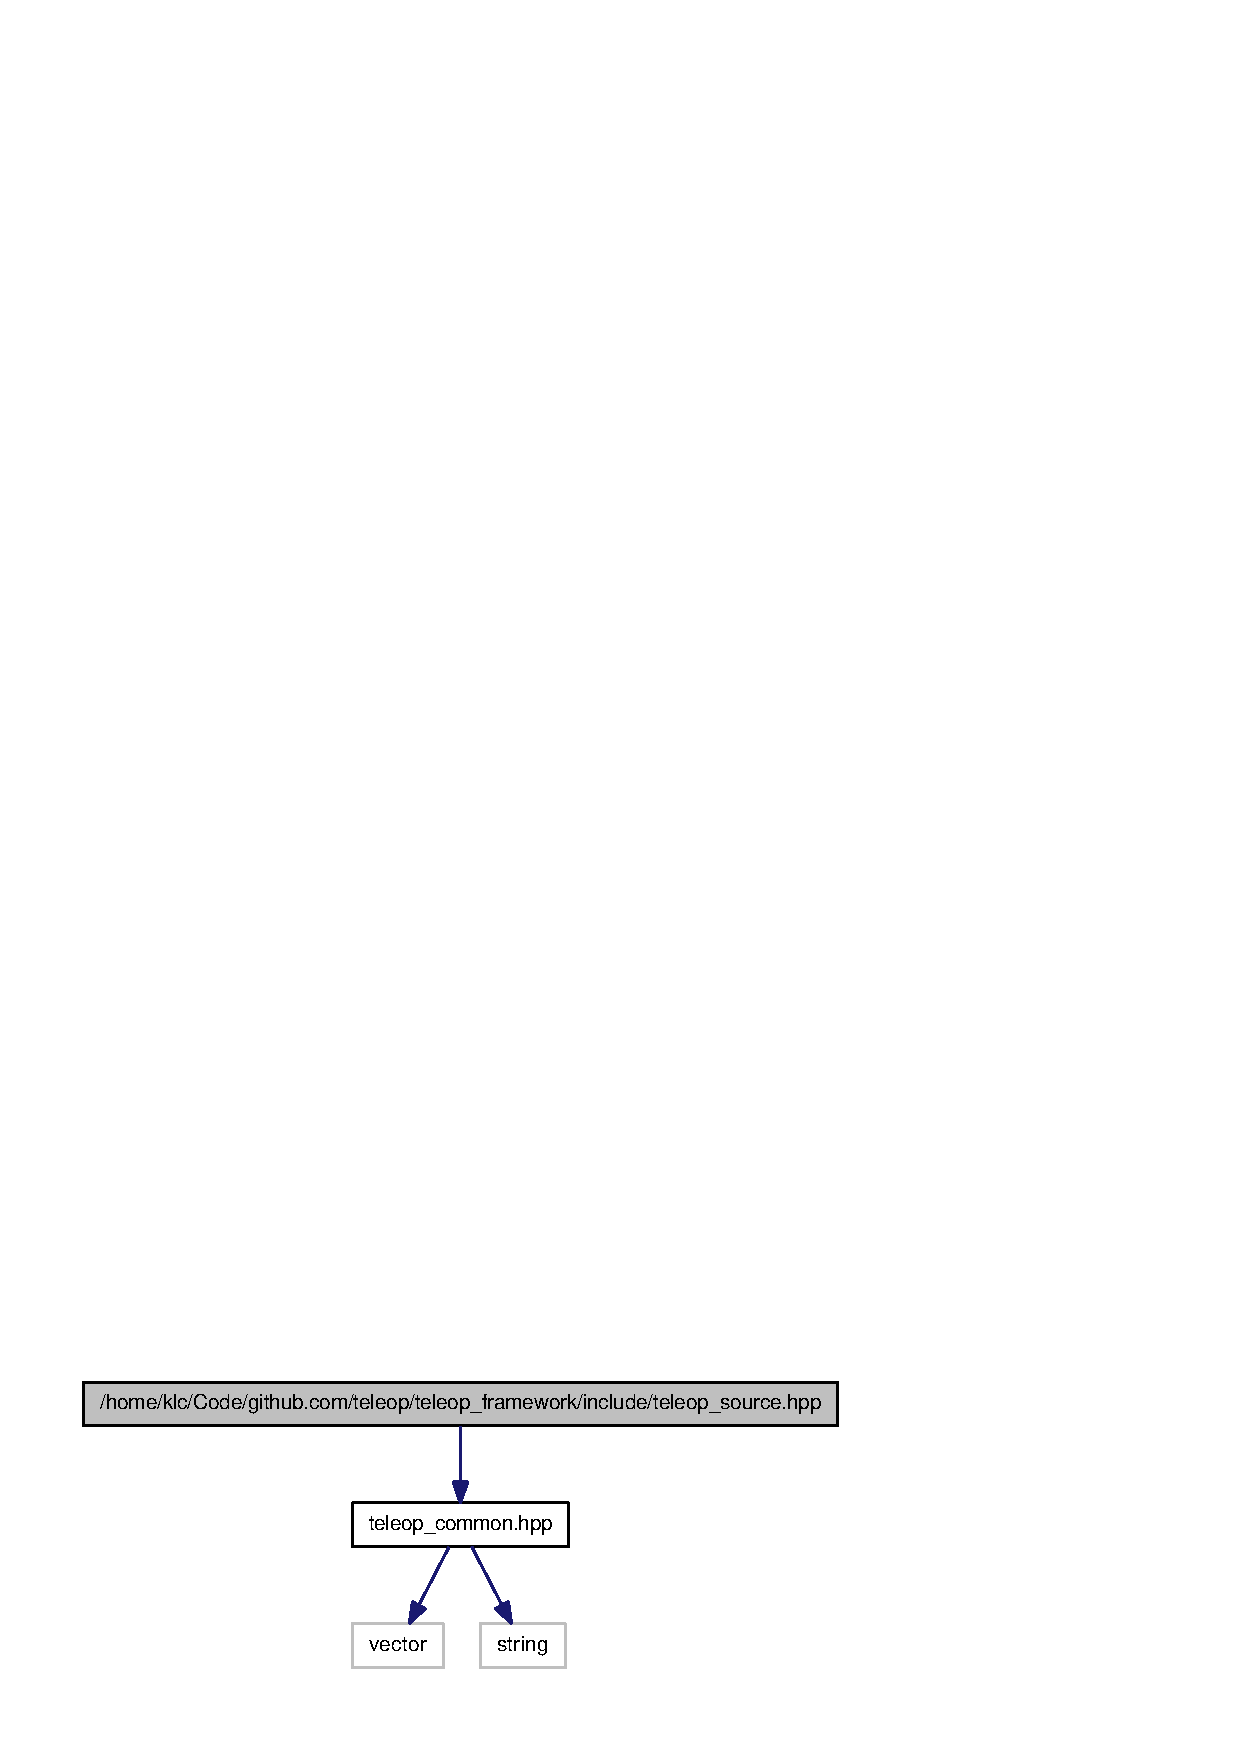
\includegraphics[width=148pt]{teleop__source_8hpp__incl}
\end{center}
\end{figure}
This graph shows which files directly or indirectly include this file:
\nopagebreak
\begin{figure}[H]
\begin{center}
\leavevmode
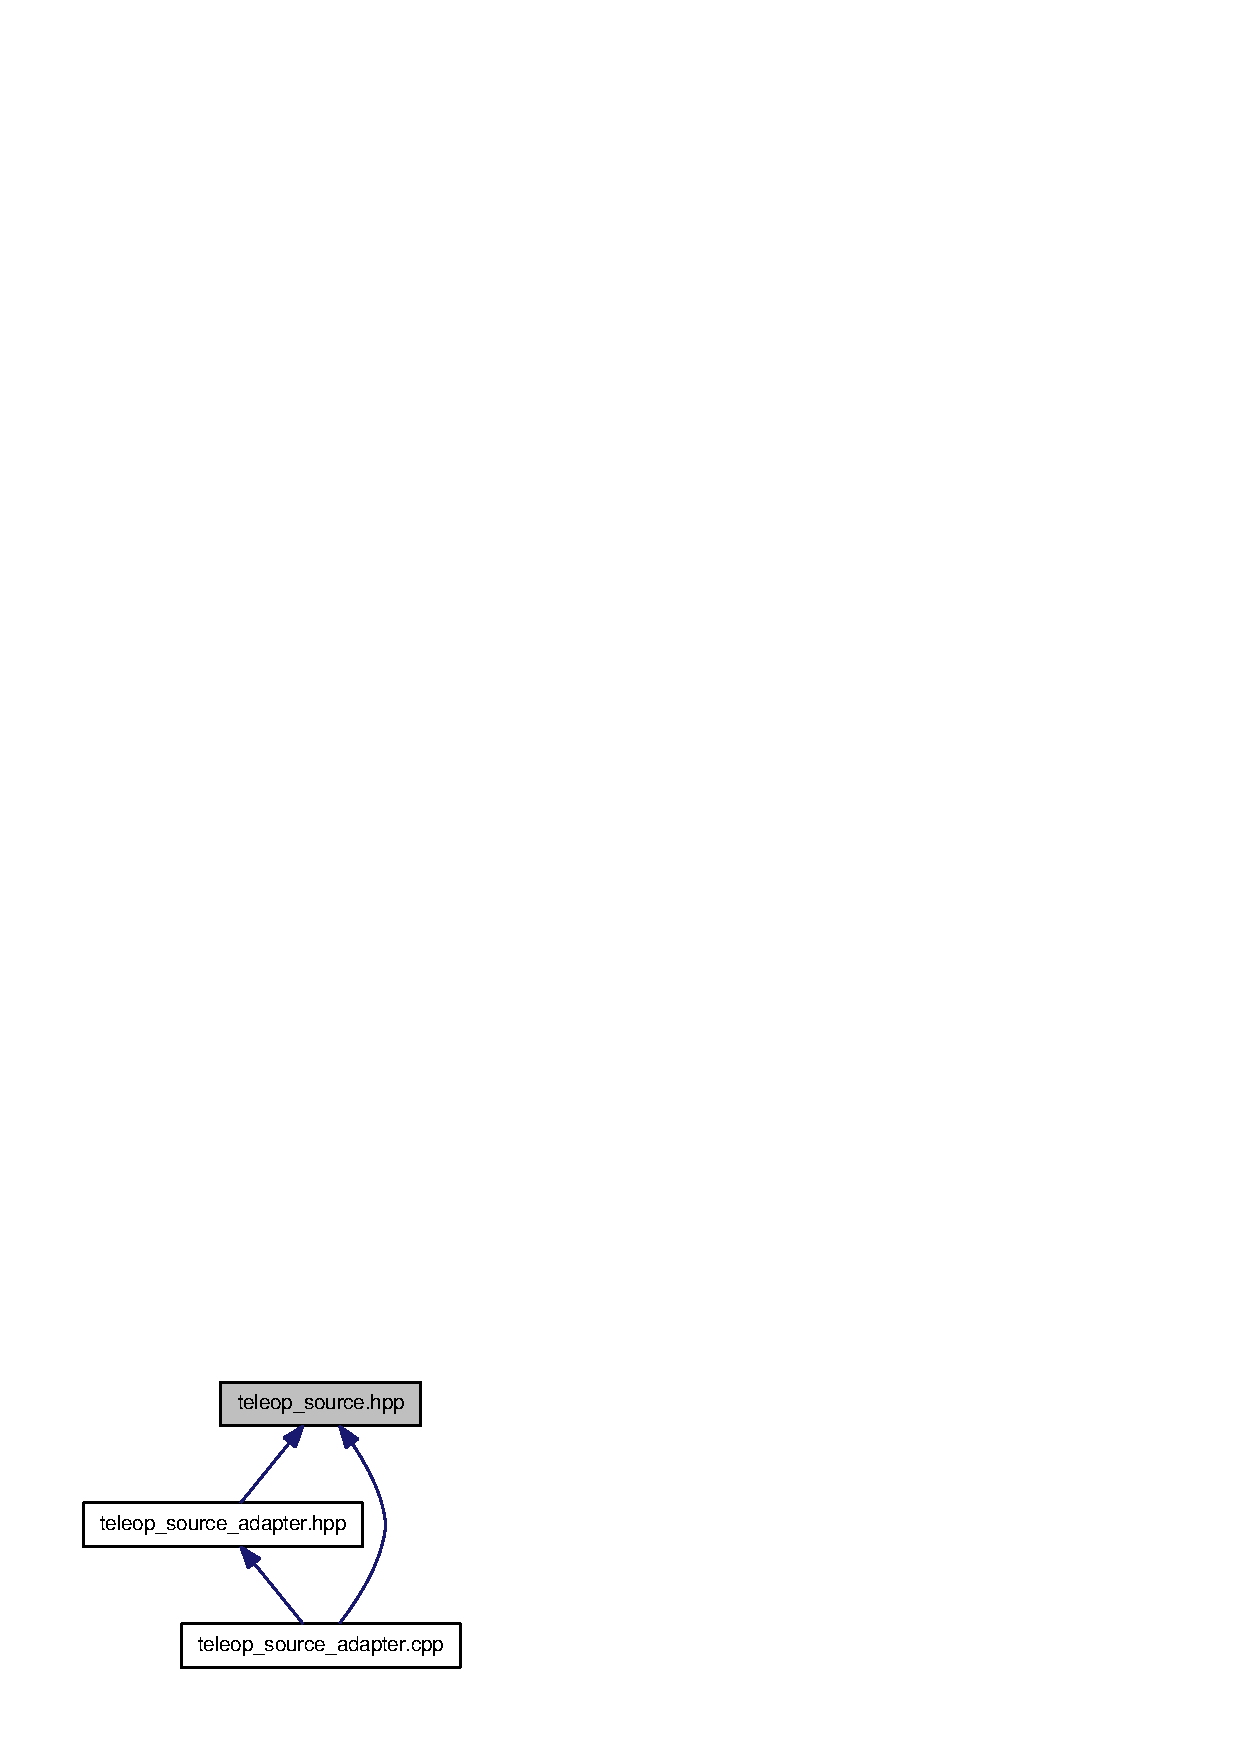
\includegraphics[width=225pt]{teleop__source_8hpp__dep__incl}
\end{center}
\end{figure}
\subsection*{Classes}
\begin{DoxyCompactItemize}
\item 
class {\bf teleop::TeleopSource}
\end{DoxyCompactItemize}
\subsection*{Namespaces}
\begin{DoxyCompactItemize}
\item 
namespace {\bf teleop}
\end{DoxyCompactItemize}

\section{teleop\_\-source\_\-adapter.hpp File Reference}
\label{teleop__source__adapter_8hpp}\index{teleop\_\-source\_\-adapter.hpp@{teleop\_\-source\_\-adapter.hpp}}
{\ttfamily \#include $<$teleop\_\-common.hpp$>$}\par
{\ttfamily \#include $<$teleop\_\-source.hpp$>$}\par
{\ttfamily \#include $<$boost/thread.hpp$>$}\par
Include dependency graph for teleop\_\-source\_\-adapter.hpp:
\nopagebreak
\begin{figure}[H]
\begin{center}
\leavevmode
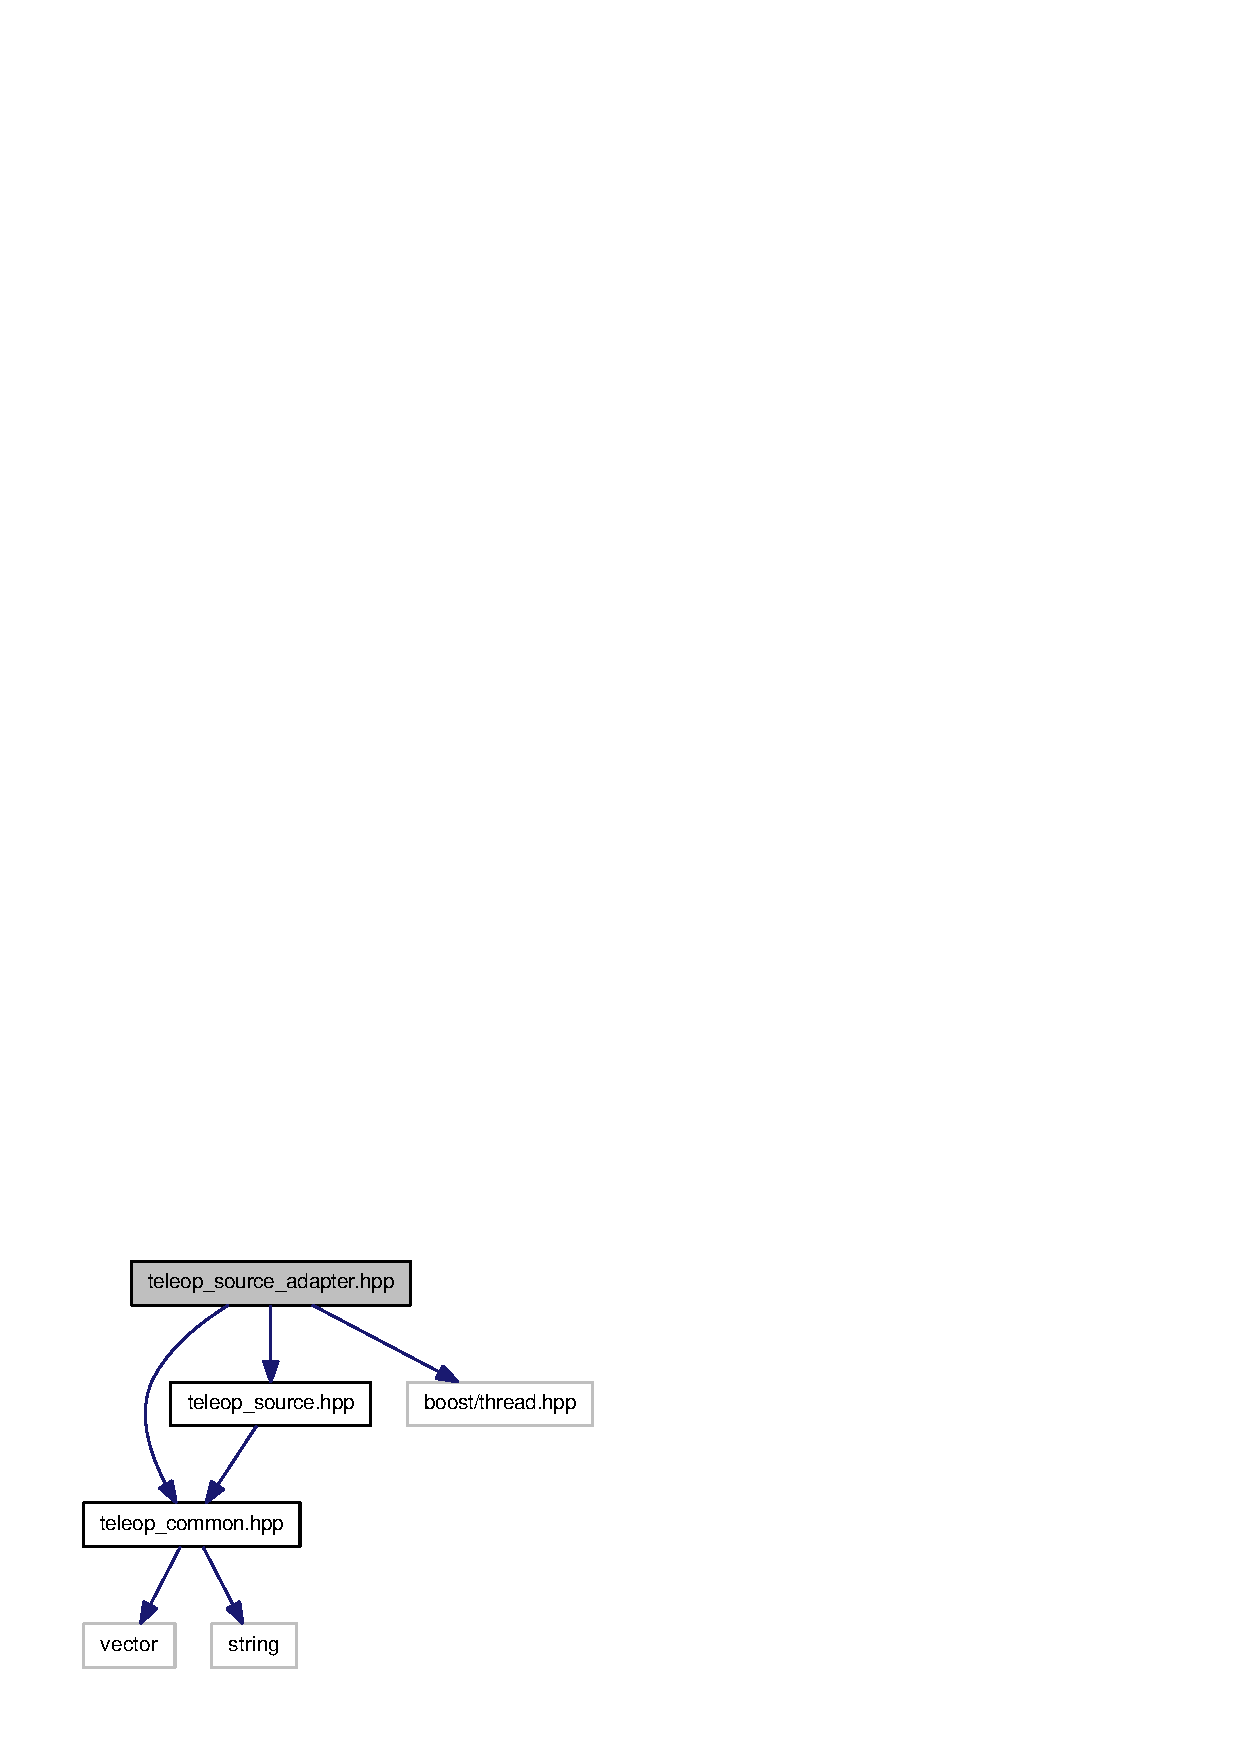
\includegraphics[width=288pt]{teleop__source__adapter_8hpp__incl}
\end{center}
\end{figure}
This graph shows which files directly or indirectly include this file:
\nopagebreak
\begin{figure}[H]
\begin{center}
\leavevmode
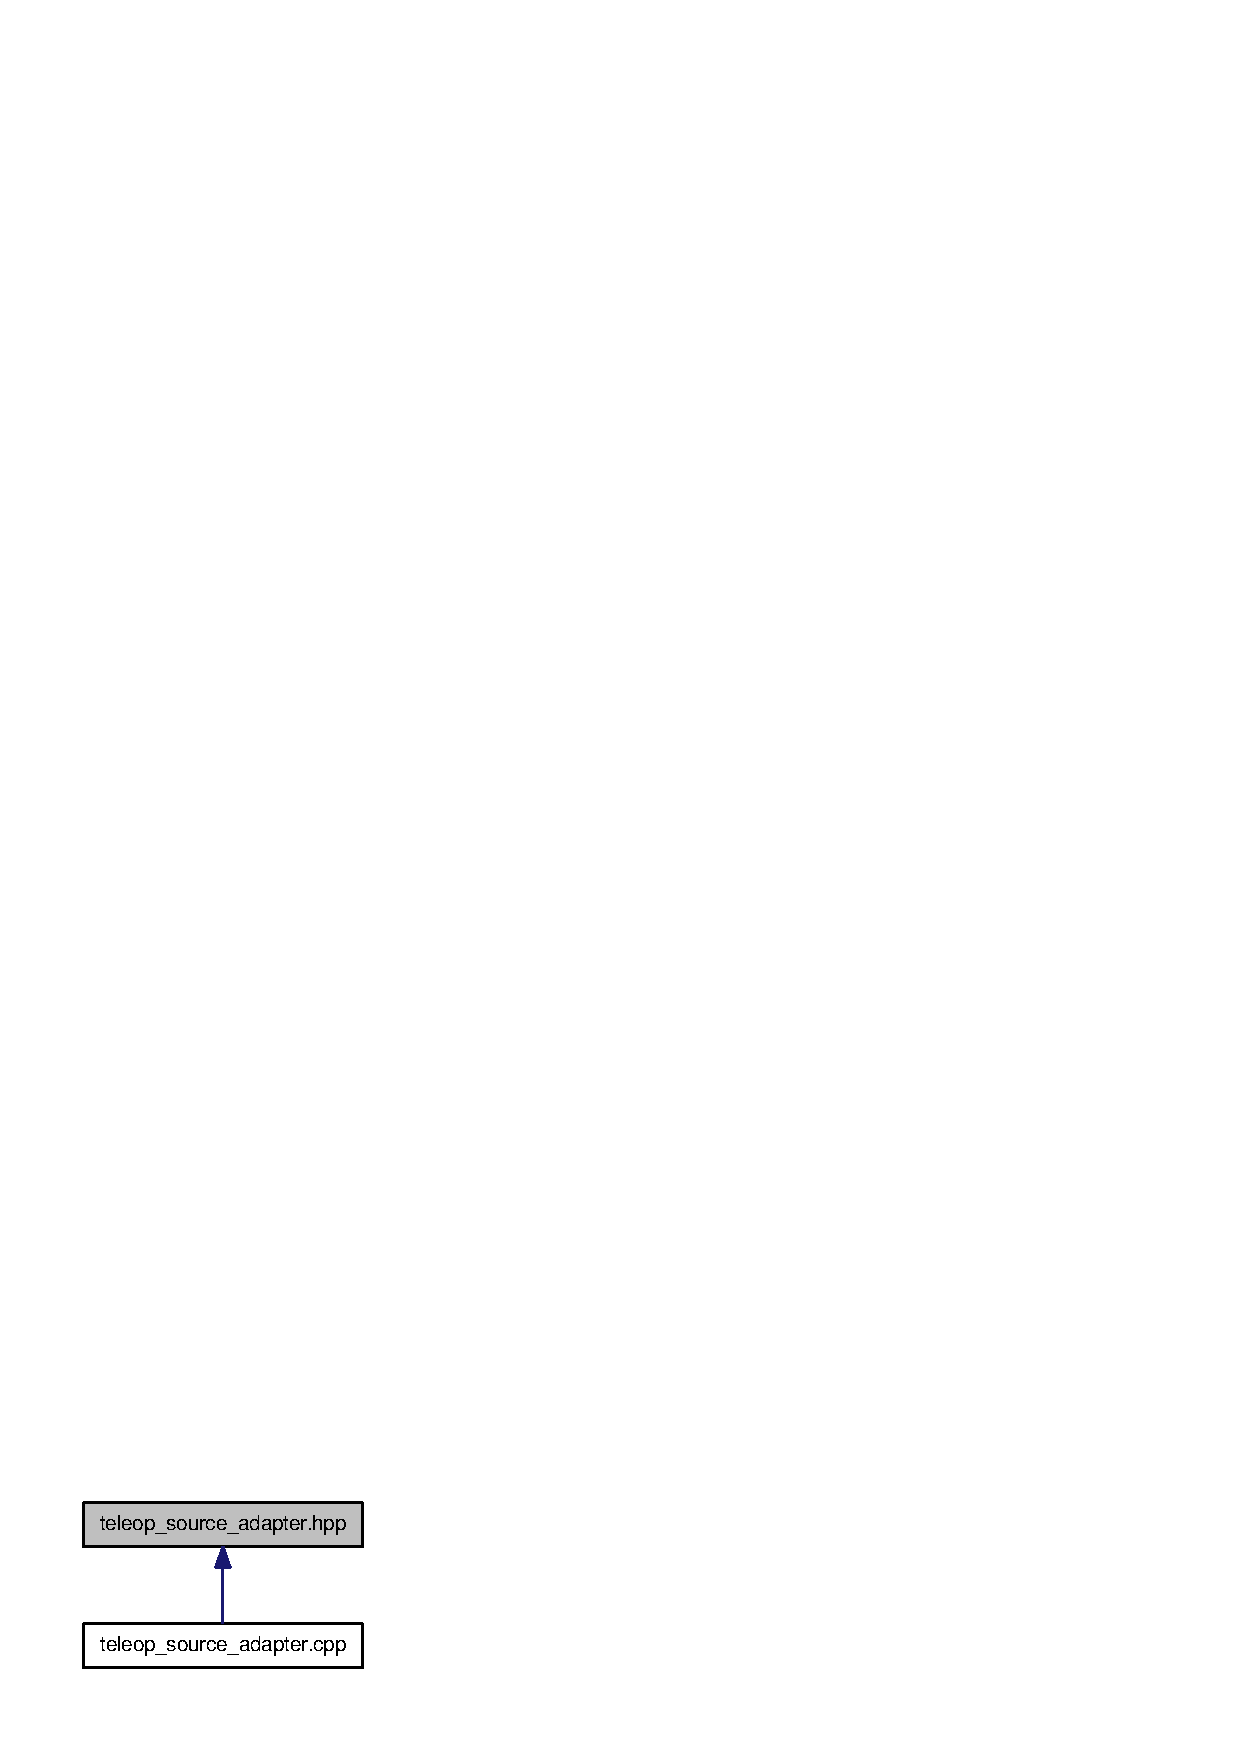
\includegraphics[width=178pt]{teleop__source__adapter_8hpp__dep__incl}
\end{center}
\end{figure}
\subsection*{Classes}
\begin{DoxyCompactItemize}
\item 
class {\bf teleop::TeleopSourceAdapter}
\item 
class {\bf teleop::TeleopSourceAdapter::TeleopSourceAdapterCallback}
\end{DoxyCompactItemize}
\subsection*{Namespaces}
\begin{DoxyCompactItemize}
\item 
namespace {\bf teleop}
\end{DoxyCompactItemize}

\section{/home/klc/Code/github.com/teleop/teleop\_\-msgs/mainpage.dox File Reference}
\label{mainpage_8dox}\index{/home/klc/Code/github.com/teleop/teleop\_\-msgs/mainpage.dox@{/home/klc/Code/github.com/teleop/teleop\_\-msgs/mainpage.dox}}

\section{teleop\_\-common.cpp File Reference}
\label{teleop__common_8cpp}\index{teleop\_\-common.cpp@{teleop\_\-common.cpp}}
{\ttfamily \#include $<$teleop\_\-common.hpp$>$}\par
{\ttfamily \#include $<$string$>$}\par
Include dependency graph for teleop\_\-common.cpp:
\nopagebreak
\begin{figure}[H]
\begin{center}
\leavevmode
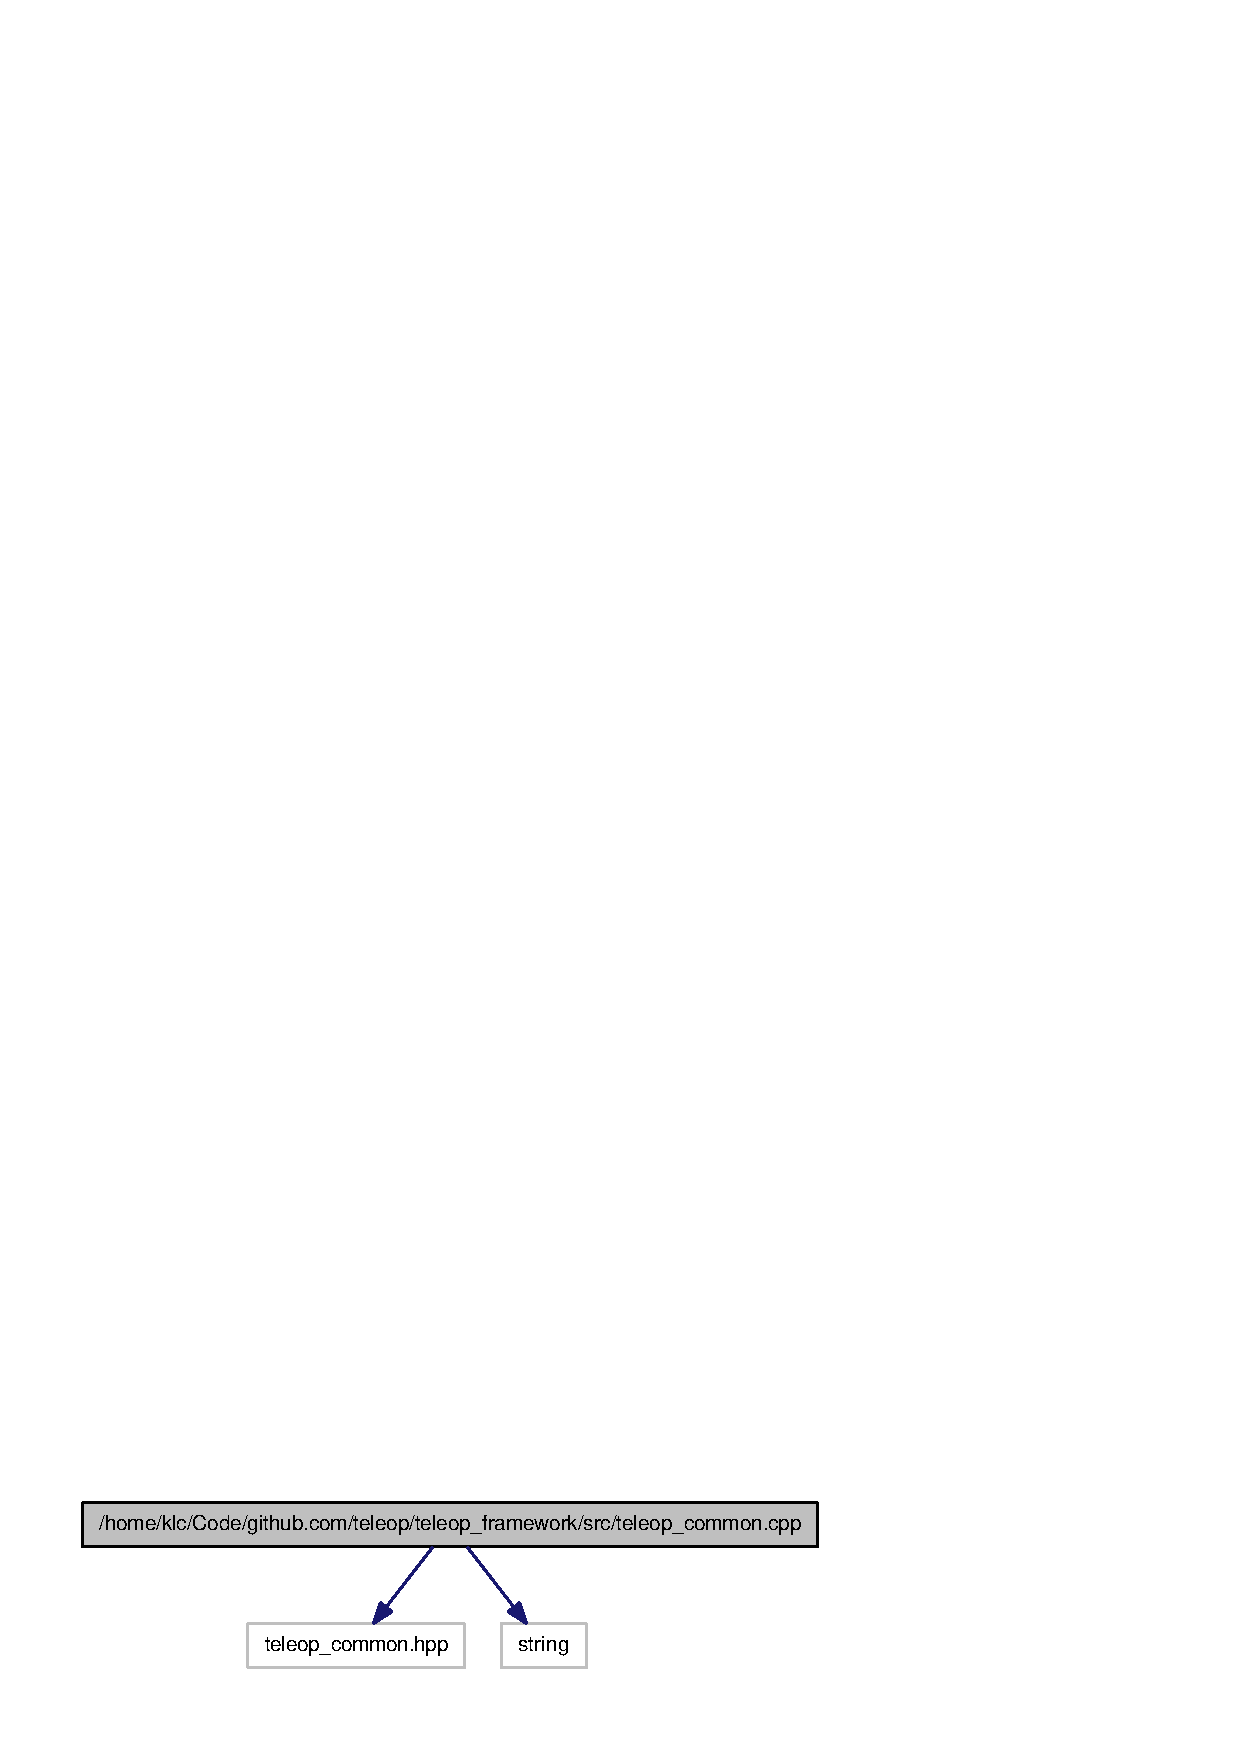
\includegraphics[width=188pt]{teleop__common_8cpp__incl}
\end{center}
\end{figure}
\subsection*{Namespaces}
\begin{DoxyCompactItemize}
\item 
namespace {\bf teleop}
\end{DoxyCompactItemize}
\subsection*{Functions}
\begin{DoxyCompactItemize}
\item 
std::string {\bf teleop::teleopAxisName} (TeleopAxisType axisType)
\item 
std::string {\bf teleop::teleopButtonName} (TeleopButtonType buttonType)
\end{DoxyCompactItemize}

\section{teleop\_\-source\_\-adapter.cpp File Reference}
\label{teleop__source__adapter_8cpp}\index{teleop\_\-source\_\-adapter.cpp@{teleop\_\-source\_\-adapter.cpp}}
{\ttfamily \#include $<$teleop\_\-common.hpp$>$}\par
{\ttfamily \#include $<$teleop\_\-source.hpp$>$}\par
{\ttfamily \#include $<$teleop\_\-source\_\-adapter.hpp$>$}\par
{\ttfamily \#include $<$boost/thread.hpp$>$}\par
{\ttfamily \#include $<$pthread.h$>$}\par
{\ttfamily \#include $<$signal.h$>$}\par
{\ttfamily \#include $<$stdio.h$>$}\par
Include dependency graph for teleop\_\-source\_\-adapter.cpp:
\nopagebreak
\begin{figure}[H]
\begin{center}
\leavevmode
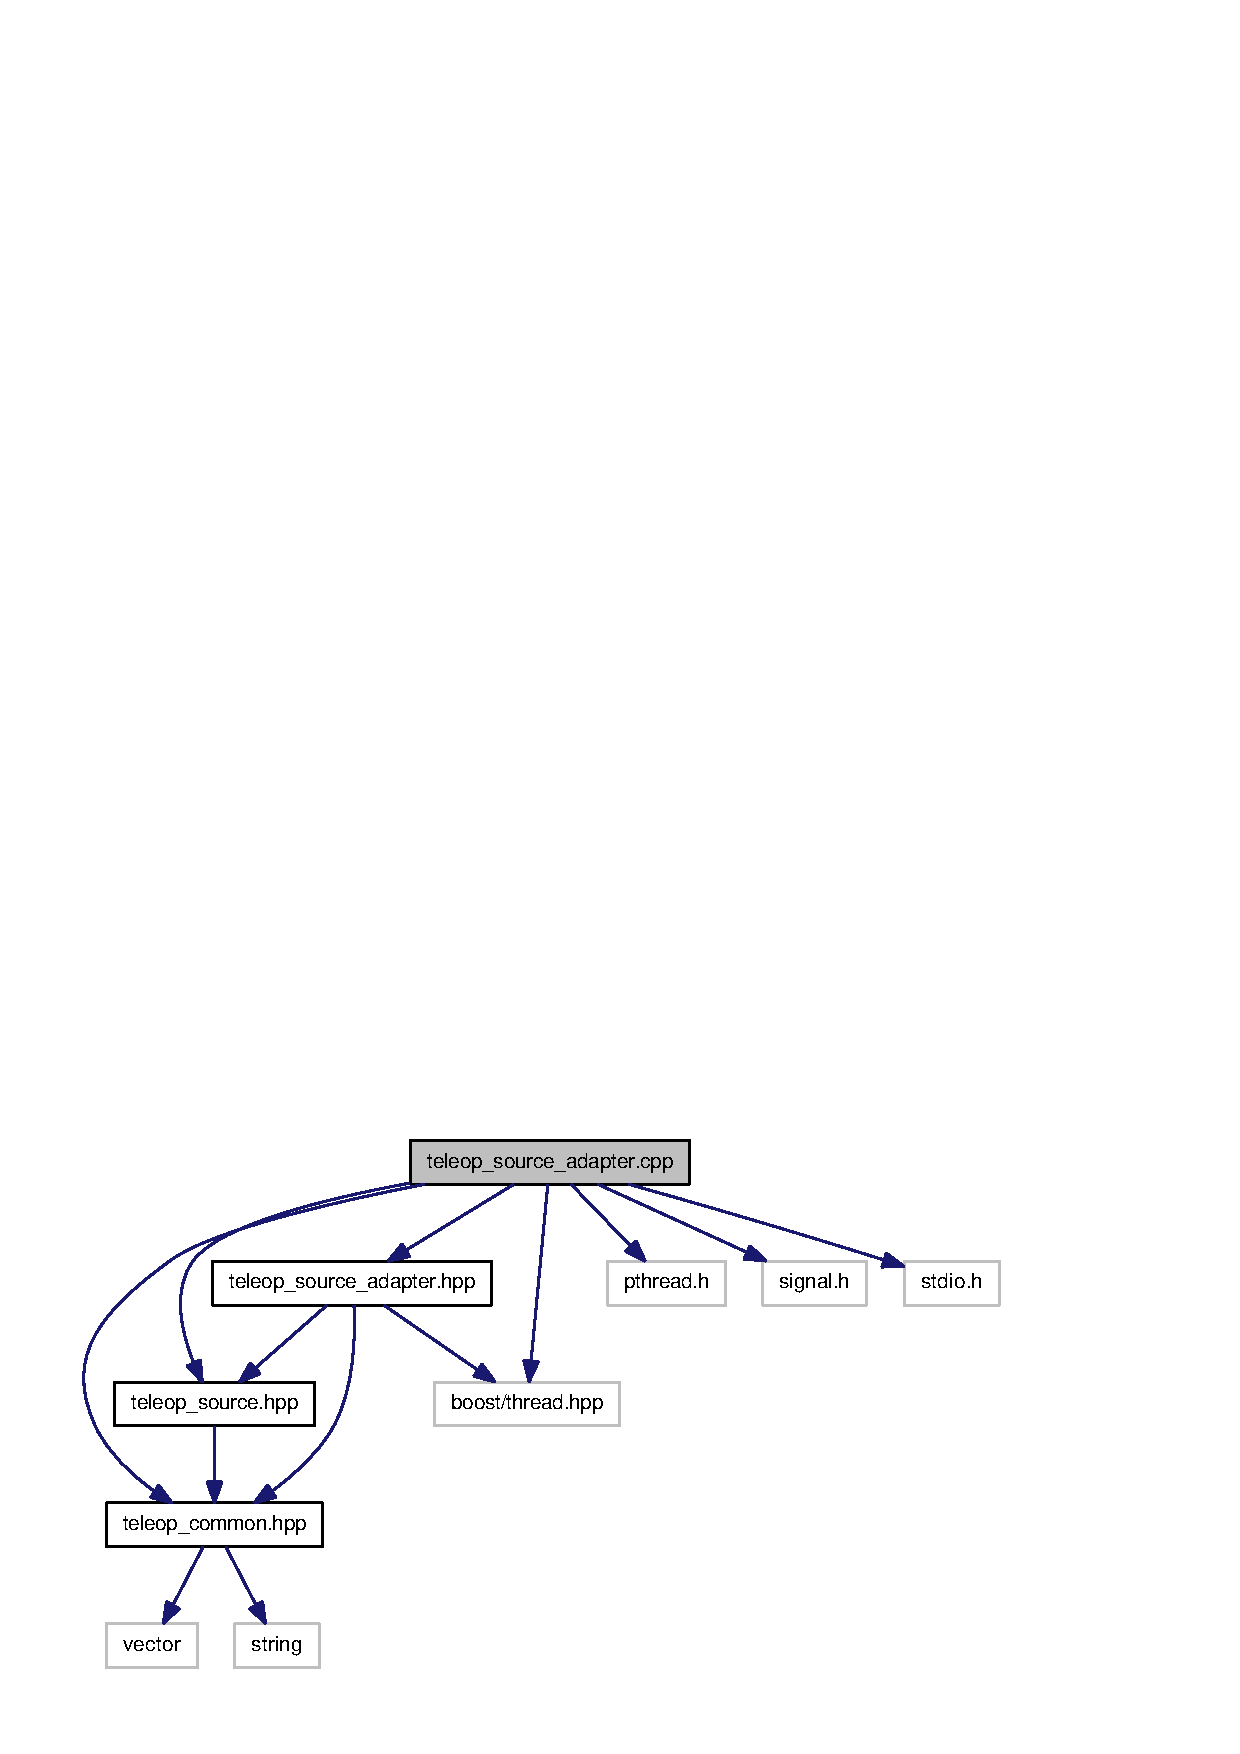
\includegraphics[width=400pt]{teleop__source__adapter_8cpp__incl}
\end{center}
\end{figure}
\subsection*{Namespaces}
\begin{DoxyCompactItemize}
\item 
namespace {\bf teleop}
\end{DoxyCompactItemize}

\printindex
\end{document}
